\definecolor{lightergray}{RGB}{247,247,247}
\definecolor{darkgreen}{RGB}{36,135,20}
\definecolor{green_comment}{RGB}{0,128,0}
\definecolor{redcell}{RGB}{238,176,176}
\definecolor{greencell}{RGB}{217,234,211}


\chapter{Diseño e Implementación de estrategias para aumentar el rendimiento de algoritmos de IA}
\label{cap:c3_implementaciones}	


	
	En este capítulo se presentan los diseños e implementaciones desarrollados a lo largo del trabajo. Inicialmente se presenta una introducción a la liberia MPI, mejorando programas sencillos fuera del ámbito de la inteligencia artificial. Posteriormente, se desarrollan los algoritmos de IA, empezando por los más sencillos y terminando por los más complejos.

%\newpage %TODO QUITAR
\section{Programas sencillos}
\label{cap:c3_1}

	Para introducir MPI en el proyecto, se implementan y comentan varios programas sencillos. Primero la multiplicación de matrices, que tiene un coste cúbico O(\(N^{3}\)), al tener que recorrer, para cada elemento de la matriz, una fila y columna entera. Segundo, algoritmos de ordenación, que para simplificar, solo se realiza un estudio de las ordenaciones con mayor complejidad temporal, O(\(N^{2}\)) y MergeSort con coste O(\(N*logN\)).


	Las matrices son un concepto matemático muy relevante en el mundo de los videojuegos y en el ámbito de la inteligencia artificial. Hay muchas técnicas de IA que conllevan la gestión de imágenes, como en el algoritmo DQN cuya red neuronal tiene como entrada varios fotogramas para poder aprender. Estas imágenes, pueden en mayor o menor medida ser implementadas con matrices.
	
	El cálculo de la multiplicación de dos matrices es cúbico O(\(N^{3}\)). Ensencialmente, es necesario recorrer toda la matriz, y para cada elemento, realizar el sumatorio de las multiplicaciones fila, columna. 
	
	Por estos motivos, es un buen primer ejemplo para presentar una estrategia basada en MPI, debido al alto coste computacional. Para ello hay que plantear cómo dividir el trabajo entre los procesos. Inicialmente, se puede pensar que es mejor enviar los datos conforme se finaliza una operación, pero en esta operación se necesitan las filas de una matriz y columnas de otra, por lo que conviene que cada proceso tenga una matriz entera en su memoria local para agilizar el proceso y poder enviar más datos al mismo tiempo. Cada \textit{worker} se va a encargar de un determinado número de filas, paralelizando así el cálculo. El \textit{master} se encarga de dividir la matriz entre los procesos. Se puede abordar con dos enfoques distintos:
	\begin{itemize}
		\item Reparto estático: los datos se dividen antes de empezar el cálculo. 
		\item Reparto dinámico: los datos se reparten en tiempo de ejecución, asignando lso mismos de forma proporcional a la velocidad de cada proceso.
	\end{itemize}



	
	
	En la primera estrategia, dividimos la matriz entre todos los \textit{workers}, dejando al \textit{master} en espera de recibir datos. Esta mejora depende de la velocidad de los procesos, pues se puede generar un cuello de botella si todos terminan y envían los datos al mismo tiempo. Además de aumentar la complejidad espacial entre los procesos, pues se divide la matriz entera entre los \textit{workers}. 
	
	En la segunda estrategia, hay un flujo constante de nuevos datos y resultados obtenidos, reduciendo el tiempo perdido en un posible cuello de botella. En la Figura \ref{fig:matrizmpi} se muestra como el \textit{master} divide la matriz, marcando en negro la parte ya procesada. A su vez cada \textit{worker} tiene una sola fila en su memoria, reduciendo la complejidad espacial.
	
	\begin{figure}[!h]
	 	\centering
	 	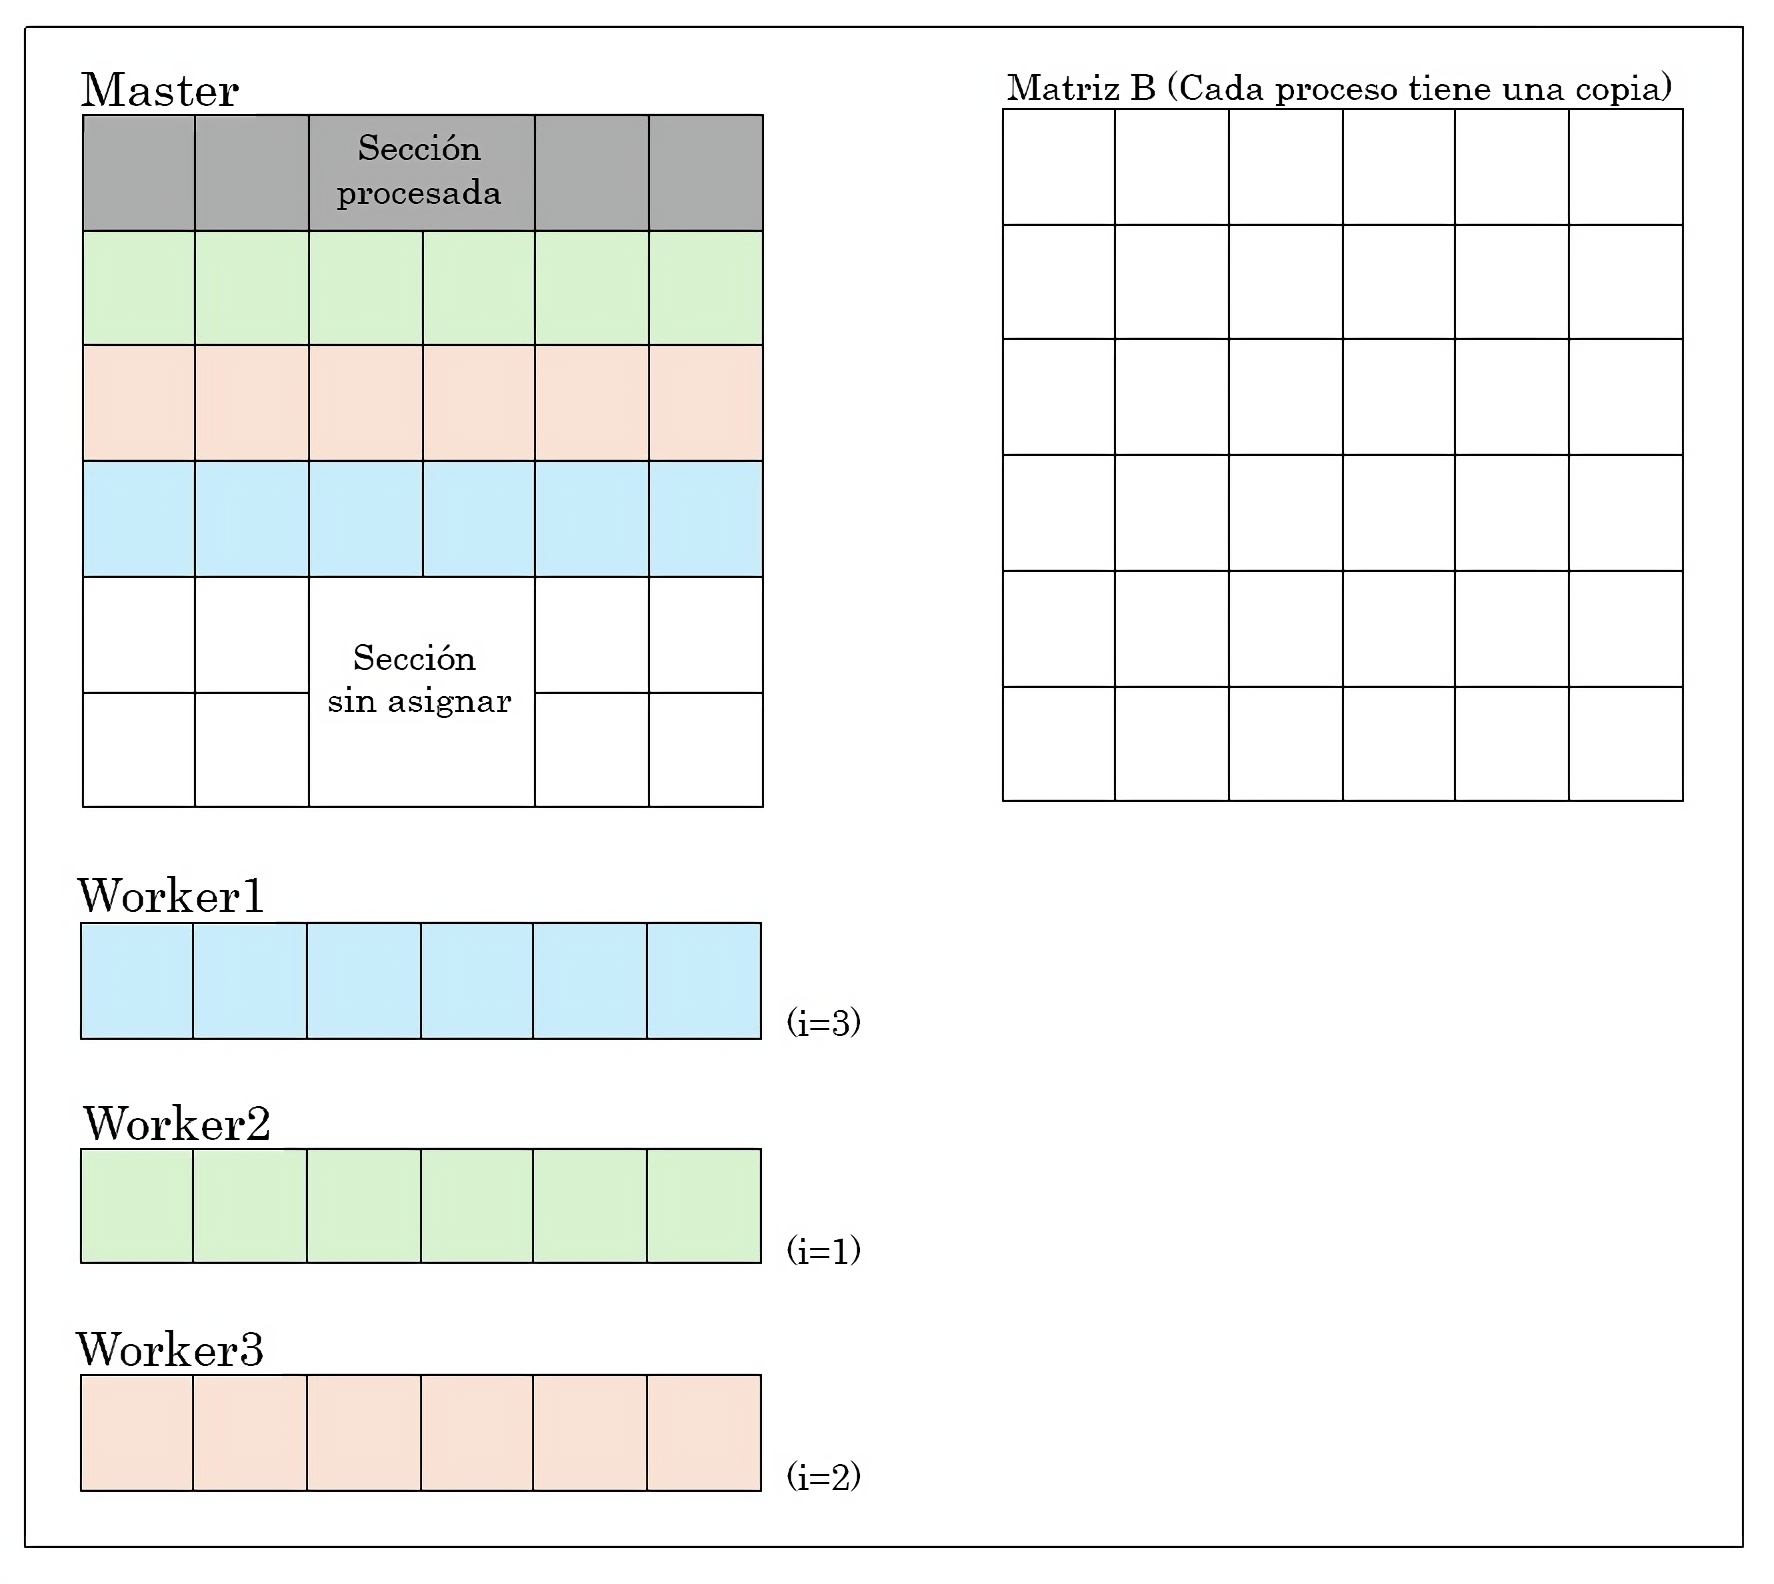
\includegraphics[width=0.58\textwidth]{images/chapter_3/matriz_mpi}
	 	\caption{División de datos entre los procesos \textit{workers} en la multiplicación de matrices}
	 	\label{fig:matrizmpi}
	\end{figure}


	%\vspace*{0.2cm}
	\newpage	
	
	Los algoritmos de ordenación tienen que iterar varias veces hasta que el array de elementos esté completamente ordenado. Y los métodos pueden variar considerablemente el tiempo de ejecución.
	
	Para las ordenaciones cuadráticas, los métodos populares como BubbleSort, InsertionSort y SelectionSort, han sido estudiados y optimizados para que, aunque tengan un coste cuadrático O(\(N^{2}\)), en el caso peor, proporcionen un buen rendimiento. Basándose en estos algoritmos, se ha diseñado uno adicional llamado SequentialSort. Este algoritmo recorre todas las posiciones del array, y para cada elemento compara todos los datos, sumando en un contador los elementos mayores que el, para calcular así su posición en el array ordenado. Una vez finalizada una iteración, se coloca el elemento en el array ordenado, si la posición actual esta ocupada es porque hay una repetición del elemento, y se tiene que colocar en la siguiente celda libre. La Figura \ref{fig:sequentialsortmpi} representa el proceso de ordenación, marcando en gris el elemento que ha de compararse con los demás en la iteración i-ésima.
	
	\newpage

	\begin{figure}[!h]
		\centering
		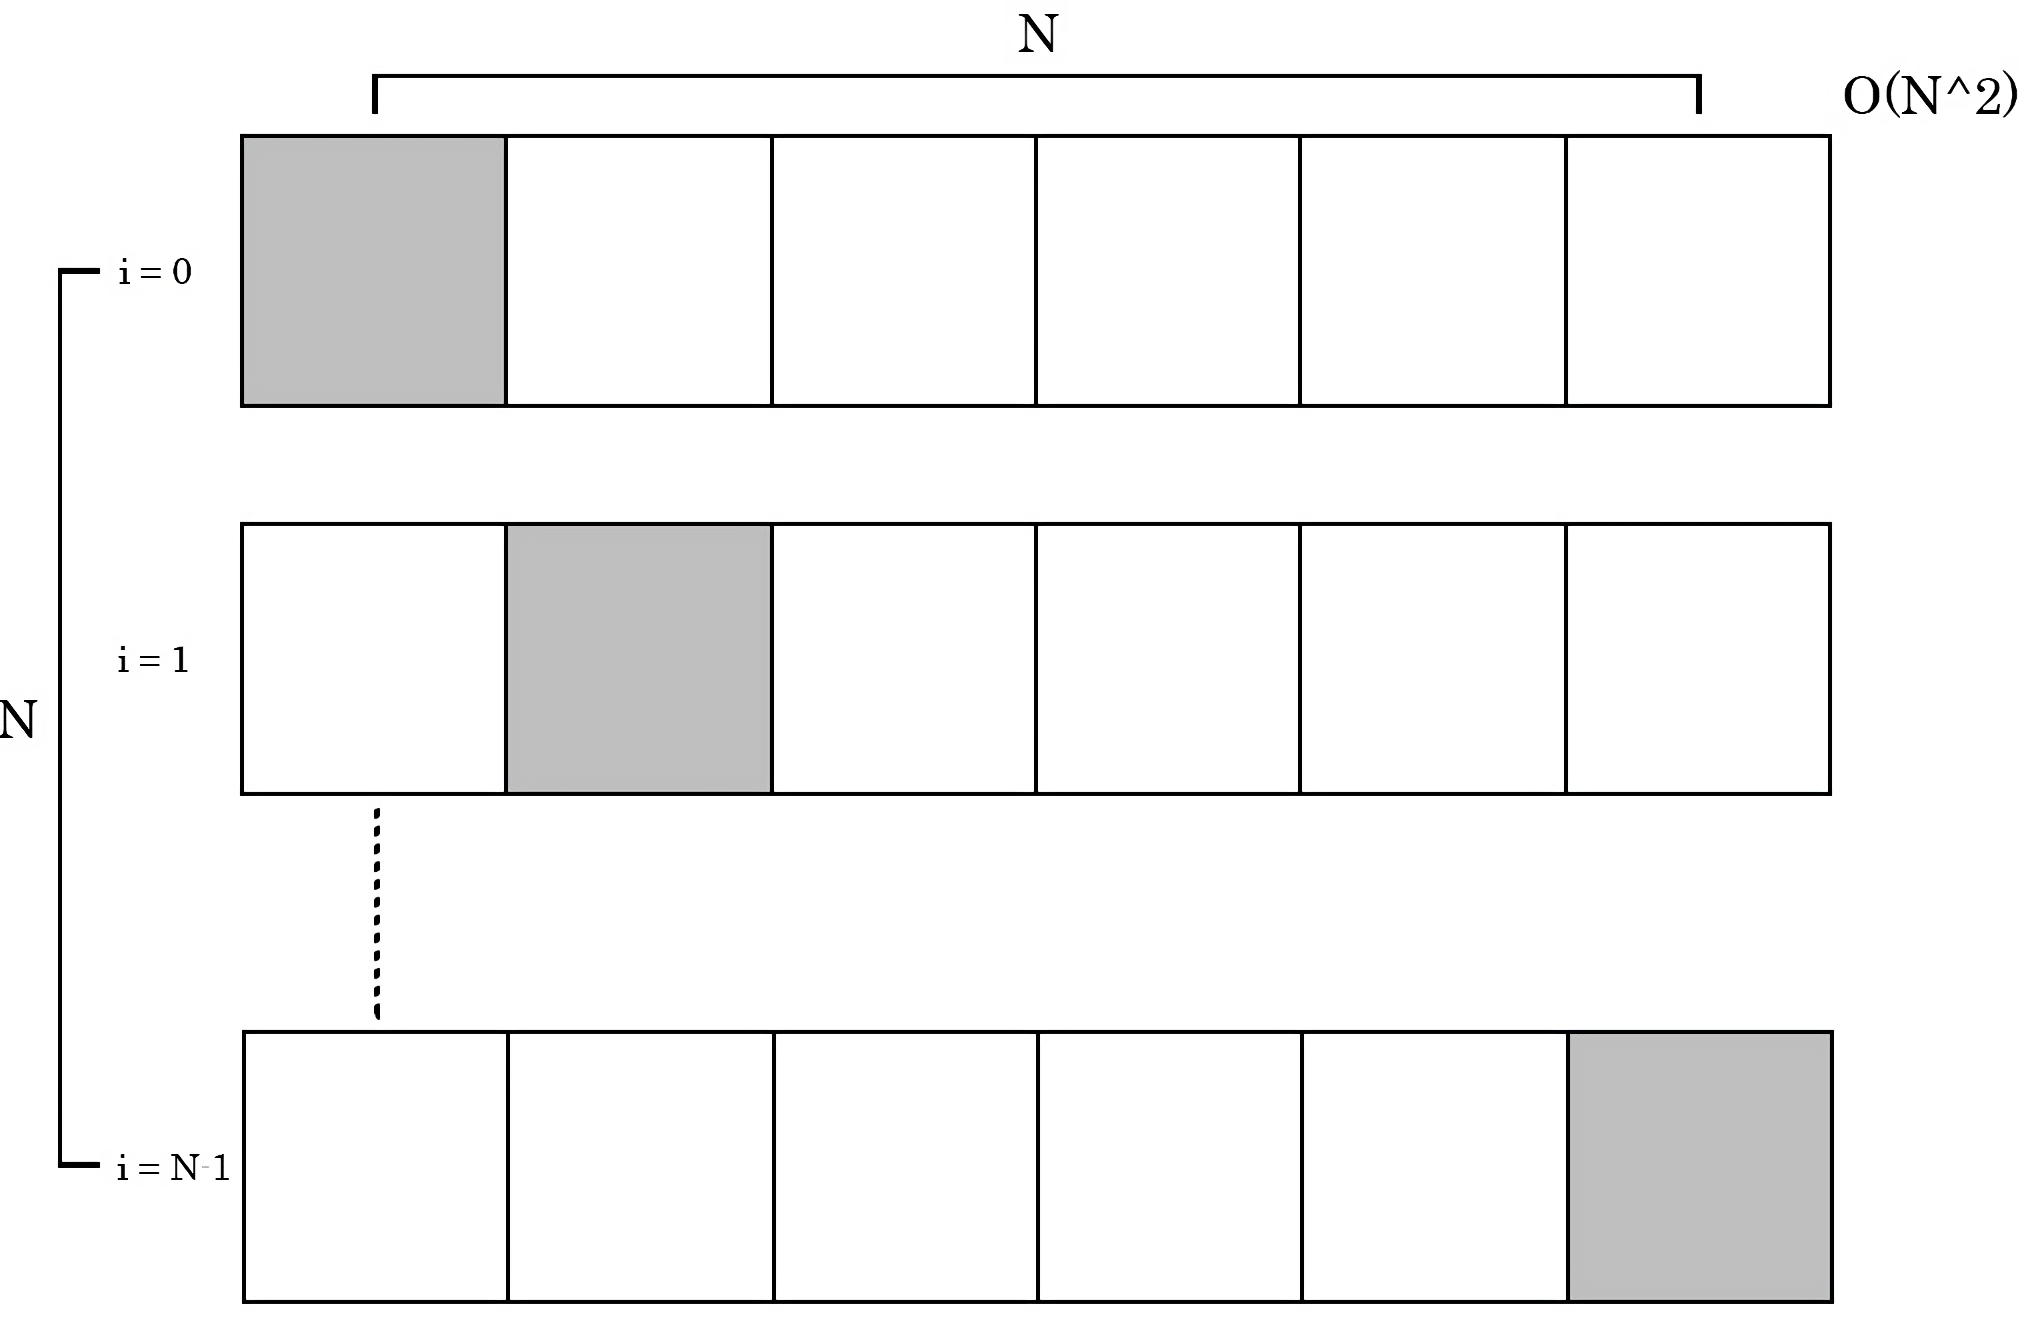
\includegraphics[width=0.6\textwidth]{images/chapter_3/sequentialsort_mpi}
		\caption{Iteraciones del algoritmo SequentialSort}
		\label{fig:sequentialsortmpi}
	\end{figure}
	
	Este método siempre tendrá coste cuadrático O(\(N^{2}\)). No es como los anteriores que van reduciendo el espacio conforme aumentan las iteraciones, pero es fácilmente paralelizable. 
	
	Para lograr reducir el tiempo de ejecución para esta ordenación cuadrática, se desarrollan las siguientes dos estrategias. Cada con sus ventajas e inconvenientes.
	
	\begin{enumerate}
		\item Enviar a todos los \textit{workers} el array entero para que trabajen de manera independiente.
		\item Dividir el array entre los \textit{workers} para trabajar conjuntamente.
	\end{enumerate}
	
	En la primera estrategia el \textit{master} envía a todos los \textit{workers} el array entero. Una vez recibido el array de elementos, el \textit{master} envía elementos sin procesar del array orginal a los \textit{workers} disponibles. Al recibir un elemento lo procesan (hacen las comparaciones), y envían la posición del elemento al \textit{master}, recibiendo de vuelta otro si todavía faltan elementos por procesar. 
	
	No obstante la segunda estrategia se logra reducir el uso de memoria de tal forma que entre todos los procesos ejecutados solo haya dos copias del array que hay que ordenar, en lugar de mantener \textit{M} copias (siendo \textit{M} el número de procesos ejecutados). En cada iteración, el \textit{master} envía un elemento a todos los \textit{workers}. Estos hacen todas las comparaciones en sus subarrays y devuelven cuantos elementos pertenecientes a su subarray son mayores que el recibido. Ambas estrategias tienen la misma complejidad temporal.



	Los algoritmos de ordenación logarítmicos son muy útiles y eficientes. QuickSort tiene varios problemas como la profundidad de recursión y en el caso peor es cuadrático. Los algoritmos de RadixSort y HeapSort son eficientes sin aplicar mejoras, y MergeSort es muy popular, tanto que se aplica en Python para el método de ordenación por defecto, TimSort\cite{auger2015merge}. Este último combina InsertionSort, una ordenación cuadrática muy eficiente para ordenar para ordenar pequeños conjuntos de datos, teniendo una baja sobrecarga en términos de operaciones. Para luego usar las mitades ordenadas con MergeSort. Sin embargo, el algoritmo básico de MergeSort no es tan eficiente.
	
	Aplicando la misma idea que TimSort, se puede mejorar el tiempo de ejecución de MergeSort, aplicando combinaciones de los métodos básicos con complejidad cuadrática y comprobar la eficiencia. Esta estrategia consiste en crear varios procesos (para mayor eficacia y simplicidad, el número de procesos tiene que ser potencia de dos), y se divide el array entre los procesos. Las fases de esta estrategia son:
	\begin{itemize}
		\item Primera fase de ordenación: cada proceso ordena su sub-array con el método de ordenación correspondiente. En el capítulo \ref{cap:c4_estudio}, se realiza un estudio de los algoritmos cuadráticos y SelectionSort es el algoritmo que mejores resultados obtiene.
		\item Segunda fase de reagrupación y ordenación: esta fase se repite hasta solo tener un proceso activo, es decir, el array esté completamente ordenado.
	\end{itemize}
	
	En la comunicación entre procesos, cada uno se conecta con el proceso activo más cercano. El proceso de mayor \textit{id} (\textit{rank}) envía su array ordenado y finaliza su ejecución. El proceso receptor se encarga de ordenar ambas mitades en una sola. Utilizando una barrera (barrier MPI), garantizamos que todos terminen al mismo tiempo. Esta mejora aplica la idea de sincronización con \textit{barrera simétrica mariposa}, técnica de sincronización que conecta los procesos dos a dos, aumentando la distancia de los procesos para que, en aproximadamente M iteraciones (\(2^{M}\) = número de procesos), todos los procesos estén sincronizados. Para la estrategia implementada, se sincronizan por orden de cercanía entre \textit{ids}. La Figura \ref{fig:mergesortmpi} muestra el proceso de sincronización. En cada iteración se finaliza la ejecución de los procesos en rojo, así hasta tener un único proceso con el array entero ordenado.  
	
	\vspace{0.2cm}
	
	\begin{figure}[!h]
		\centering
		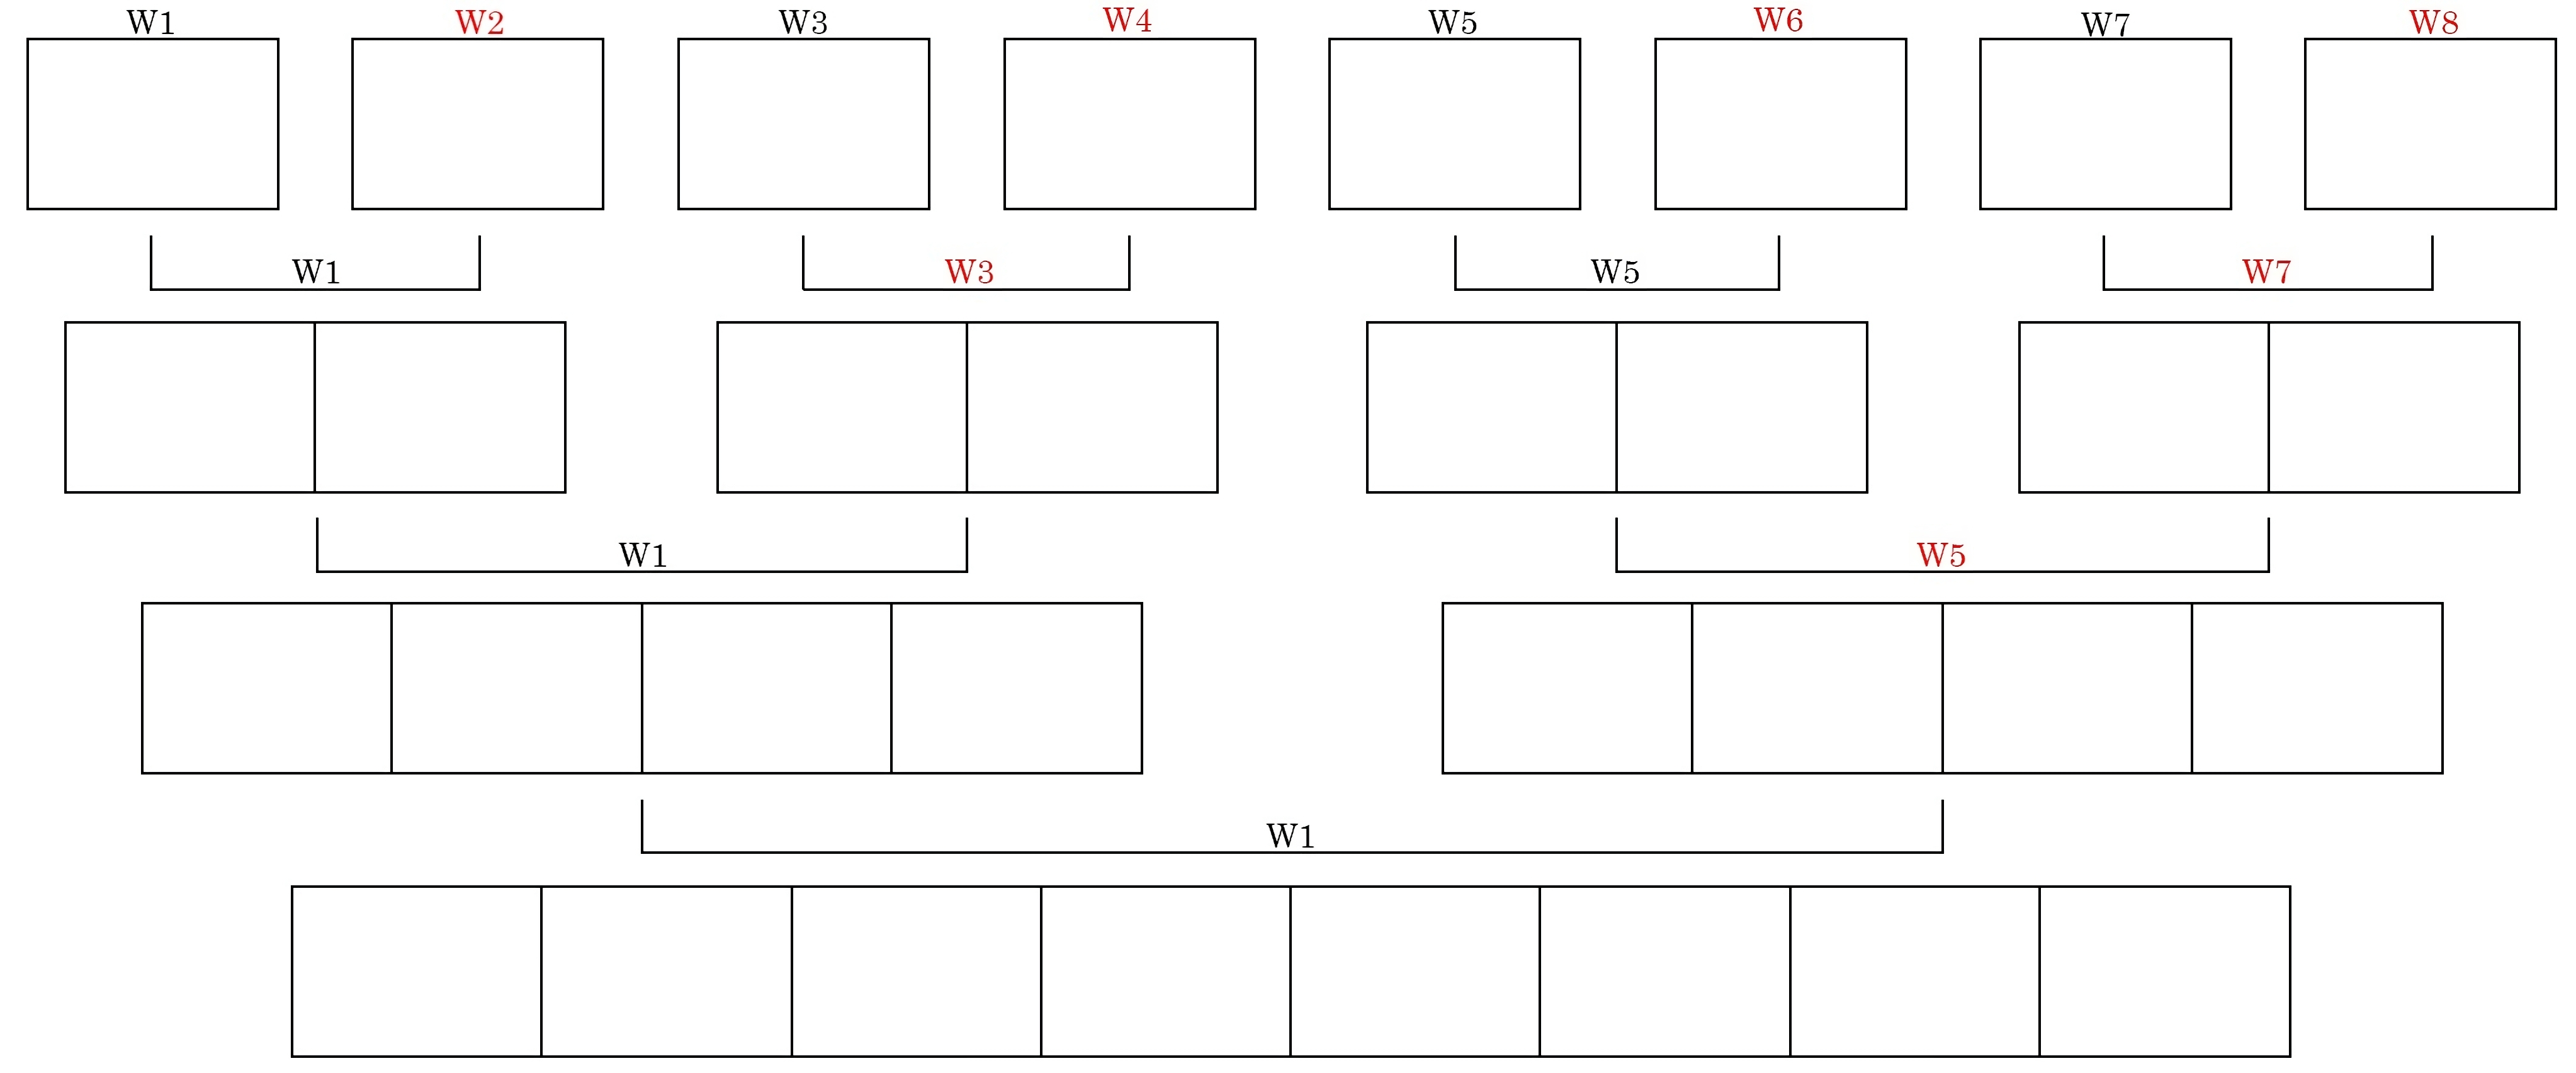
\includegraphics[width=0.85\textwidth]{images/chapter_3/mergesort_mpi}
		\caption{Ejecucion de MergeSort con 8 procesos \textit{worker} \(W_{1}\) ... \(W_{8}\)}
		\label{fig:mergesortmpi}
	\end{figure}

	\begin{comment}[!h]
		\centering
		
		
		\begin{subfigure}[t]{0.33\textwidth}
			\centering
			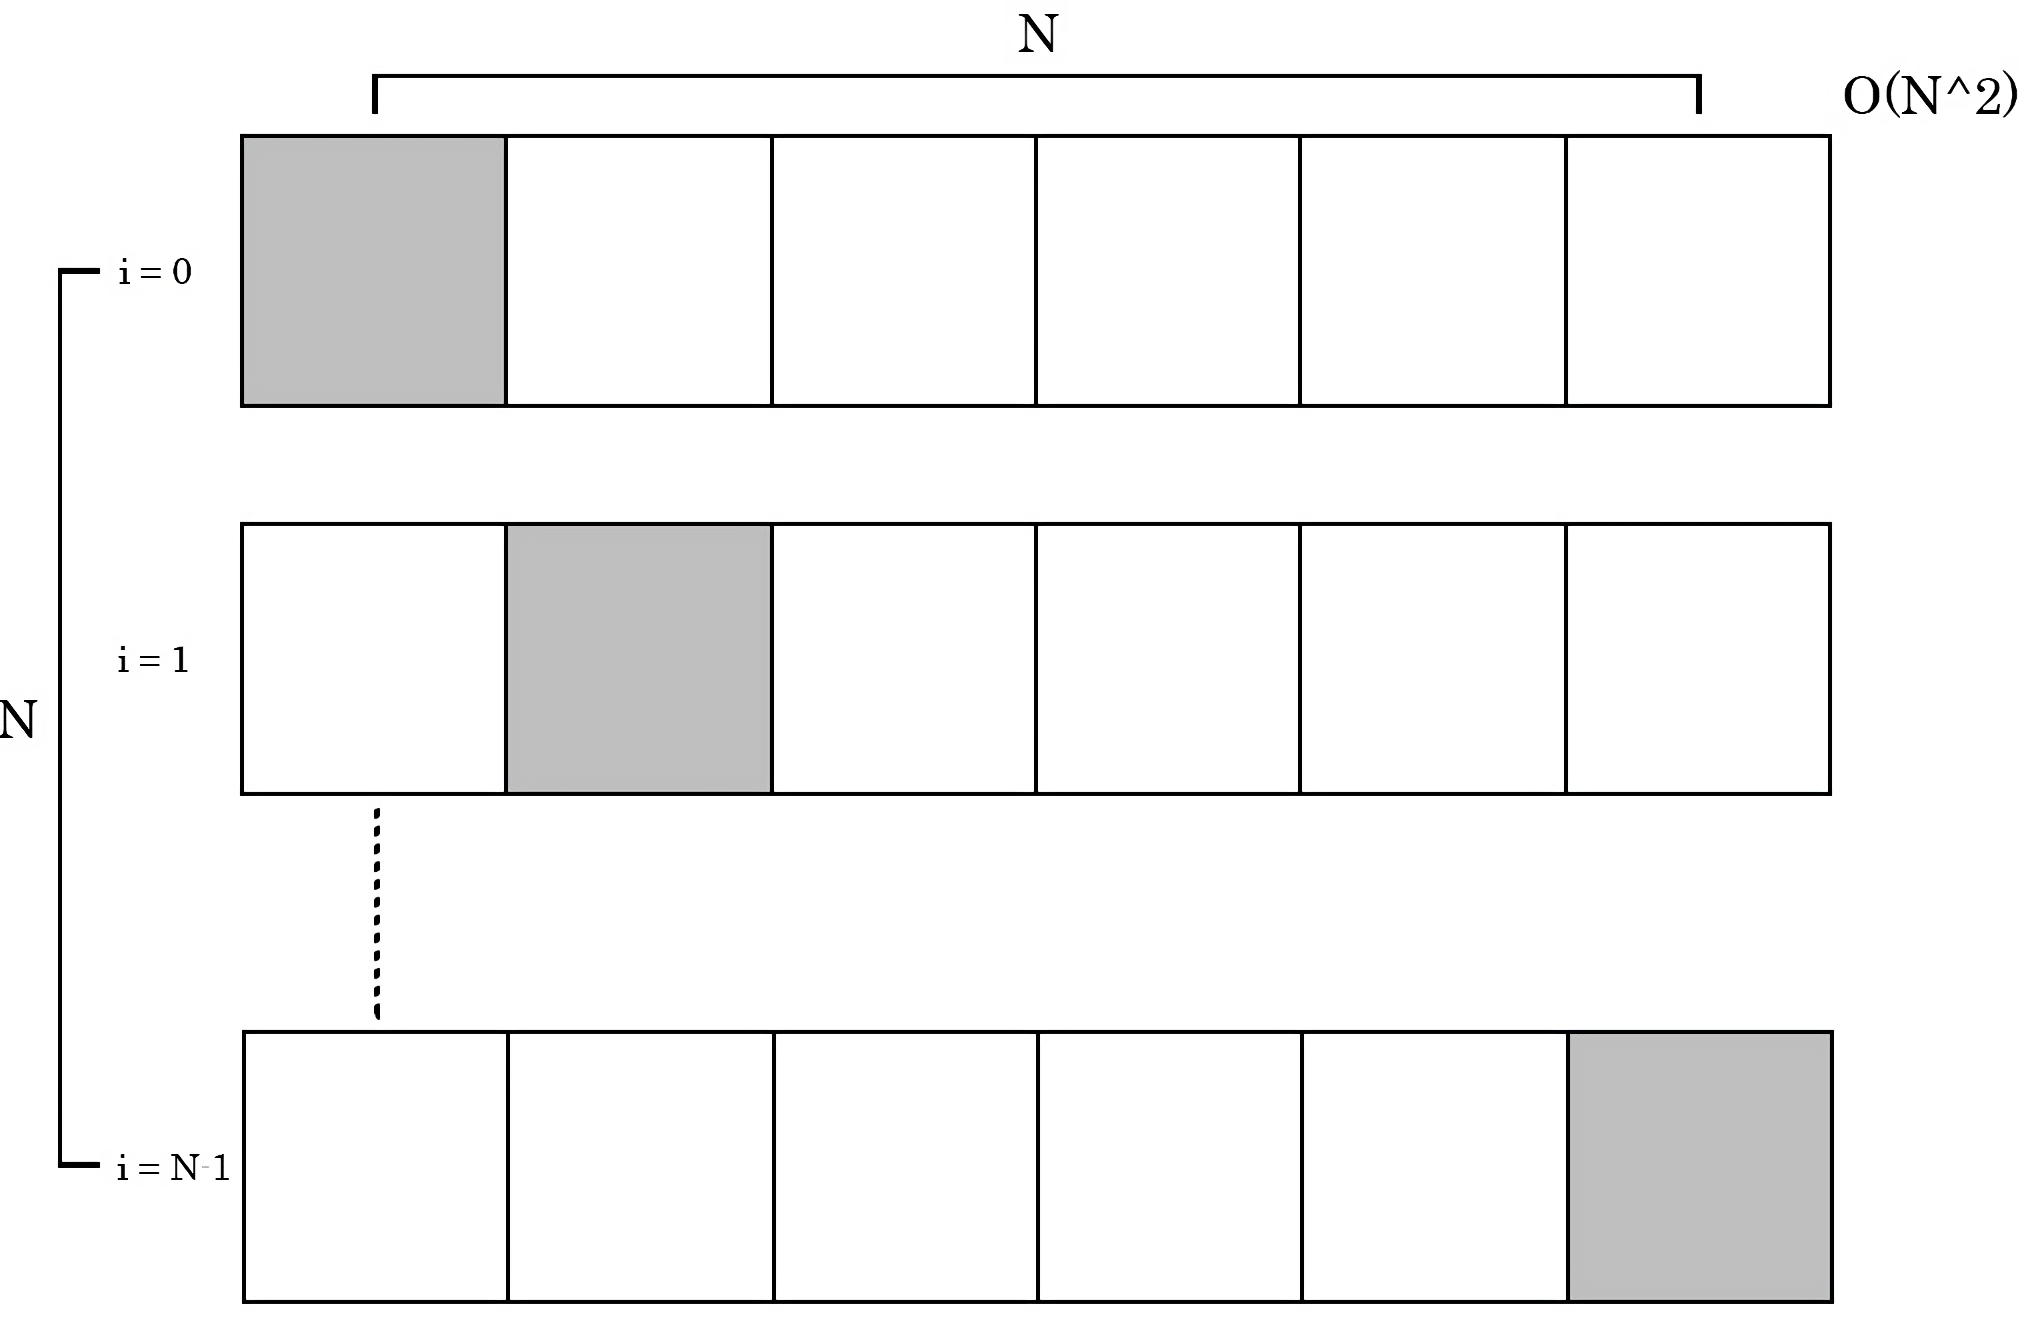
\includegraphics[width=\textwidth]{images/chapter_3/sequentialsort_mpi}
			\caption{MPI - SequentialSort}
			\label{}
		\end{subfigure}
		\hfill
		\begin{subfigure}[t]{0.48\textwidth}
			\centering
			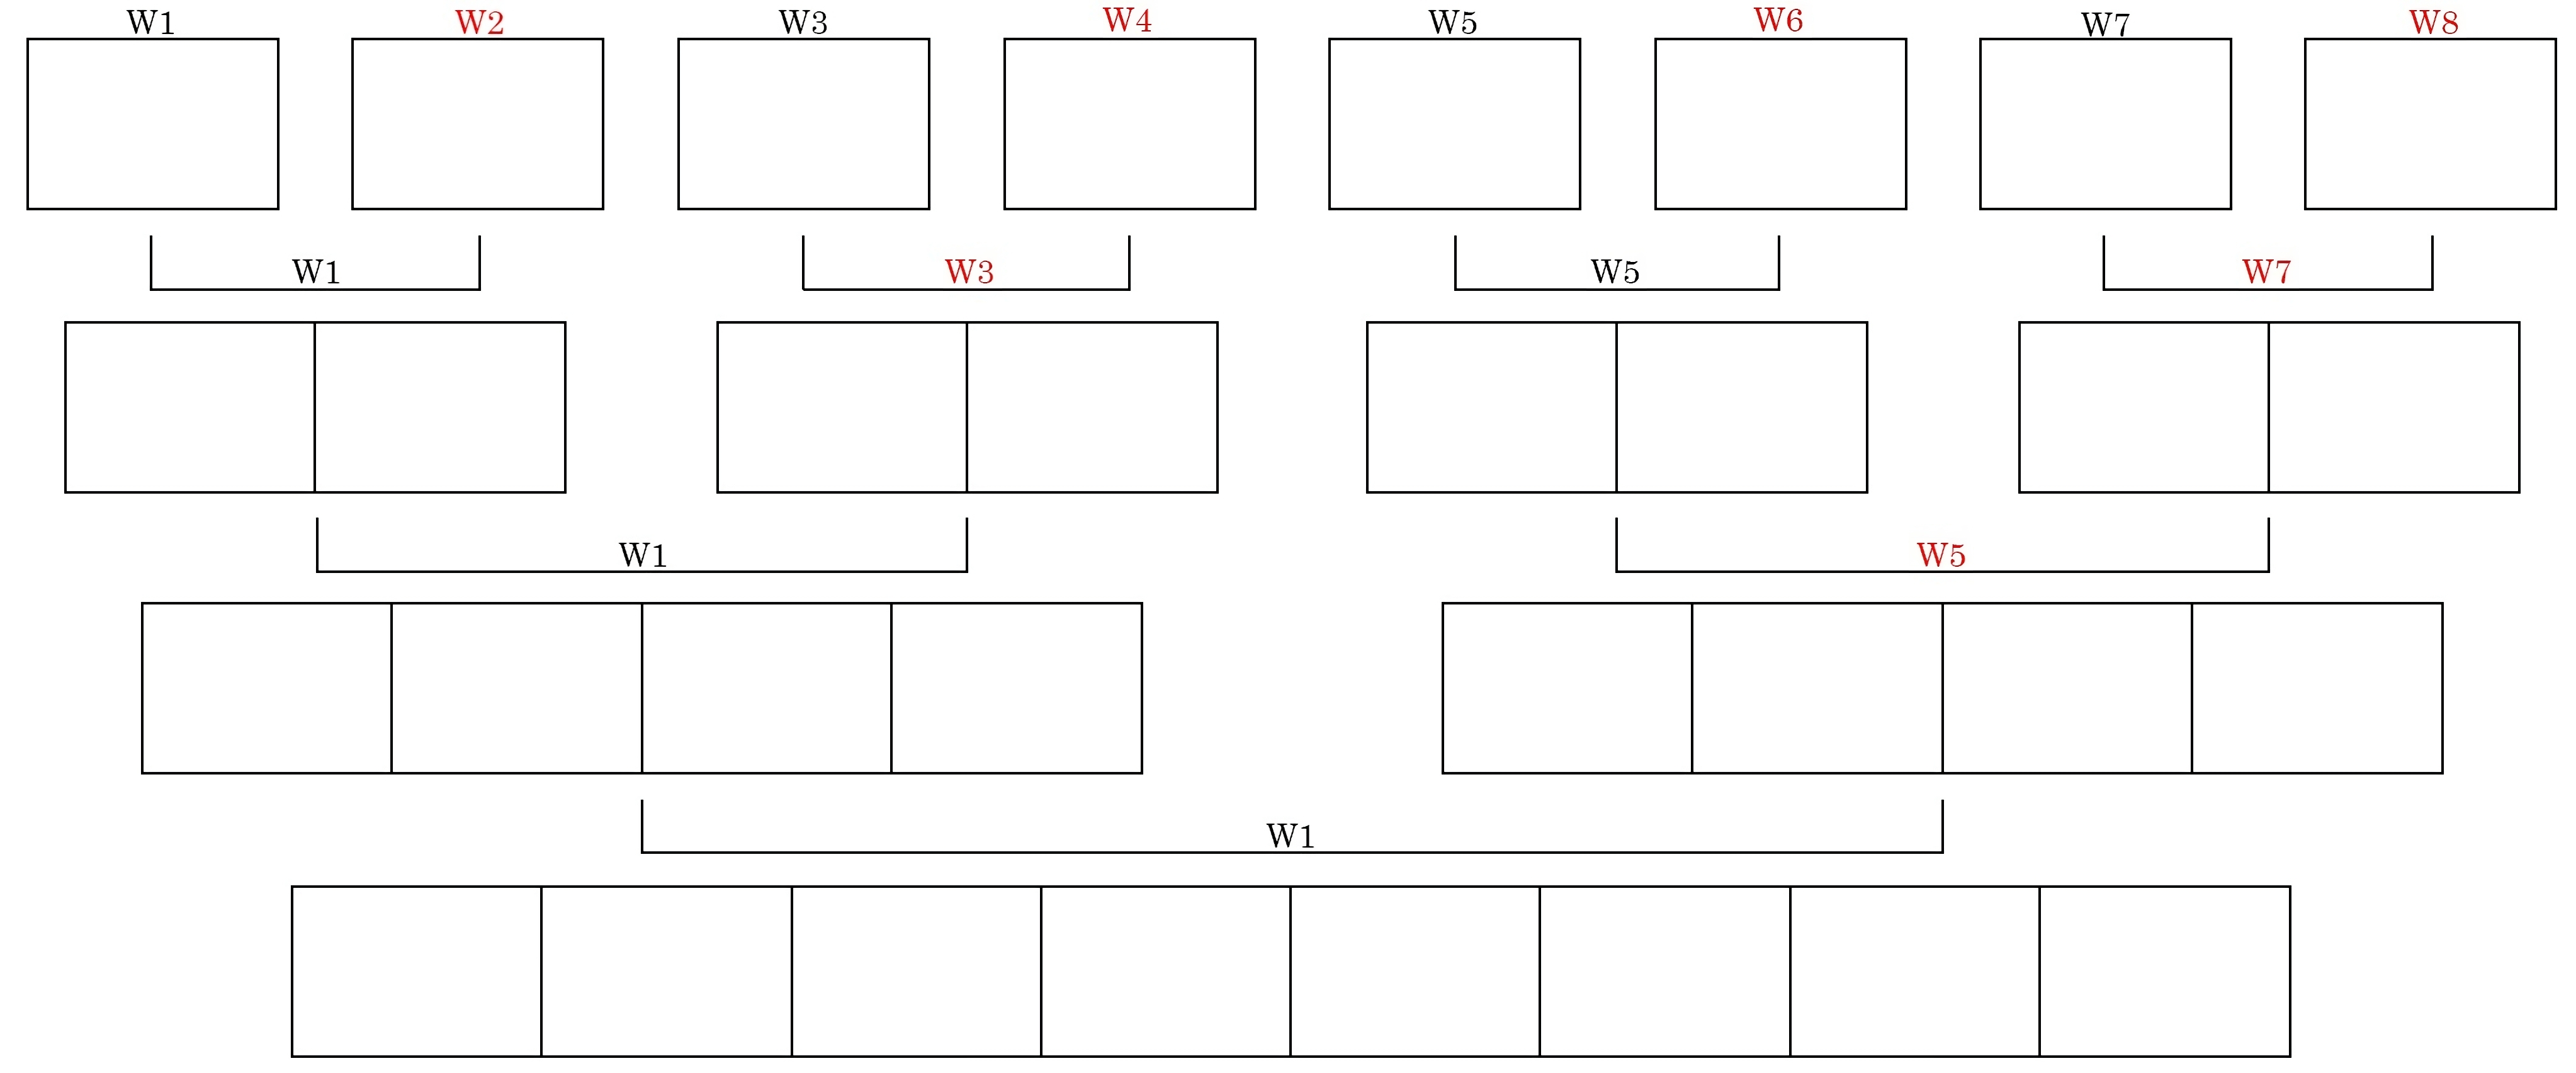
\includegraphics[width=\textwidth]{images/chapter_3/mergesort_mpi}
			\caption{MPI - MergeSort}
			\label{}
		\end{subfigure}
		
		\caption{Mejoras MPI de las ordenaciones}
		\label{}
	\end{comment}

	
	Para aplicar MPI y paralelizar programas hay que tener en cuenta que la comunicación entre procesos requiere un tiempo para enviar/recibir mensajes. Si queremos reducir el tiempo de ejecución de un programa tenemos que asegurarnos que la estrategia es viable para mejorar el rendimiento. Si ejecutamos, por ejemplo, una búsqueda lineal en un array, a primera vista, reducir el espacio de búsqueda puede ser beneficioso. Dividiendo el espacio de búsqueda entre los \textit{workers} reduce el tiempo de O(N) a O(N/numWorkers). Pero ¿se puede reducir el tiempo de ejecución al dividir el espacio entre los \textit{workers}? 
	
	Para responder esta pregunta es necesario tener en cuenta el tiempo de paso de mensajes (overhead). Si no se tuviese en cuenta, se podría garantizar la reducción, pero la comunicación entre procesos tiene un coste, y con un tiempo lineal, generalmente no se pueden lograr mejoras, más bien aumenta el tiempo de búsqueda. 
	
	Por este motivo, hay que tener en cuenta la complejidad temporal de los algoritmos que queremos optimizar, ya que no siempre es eficiente aplicar paralelismo.


\section{Algoritmos de Clustering}

	Una vez introducido MPI con programas básicos, podemos presentar las implementaciones de los algoritmos relacionados con la inteligencia artificial. Las técnicas de clustering toman una población y, dependiendo del conjunto de datos, categoriza los individuos. Los algoritmos pueden ser supervisados, si ademas de la población a categorizar, tenemos un población categorizada previamente, o no-supervisados, si no contamos con esta población etiquetada.

	\subsection{Jerárquico Aglomerativo}
	\label{cap:3_2_1}
		Este algoritmo de aprendizaje no supervisado usa una matriz para calcular las agrupaciones. Como es una matriz simétrica, podemos reducir la complejidad espacial usando solo el triángulo superior. 
		
		La distancia entre clusters es muy importante. Además de calcular agrupaciones distintas, también varía la complejidad temporal. La más eficaz y rápida es la de centroides, para calcular la distancia entre dos cluster solo necesita el cálculo entre dos puntos (los centros de los clusters). El calculo de la distancia por enlace simple y completo, es más complejo. Cada cluster almacena las coordenadas de sus individuos, para, a la hora de calcular la distancia entre dos clusters (\(C_{i}\) y \(C_{j}\)), comprobar la distancia de cada par de puntos (donde uno pertenece a \(C_{i}\) y el otro a \(C_{j}\)). La nueva distancia usando enlace simple es la mínima distancia entre cualquier par de puntos, mientras que la completa es la máxima.
		
	
		Una vez comentadas las estrategias en el cálculo de multiplicación de matrices, podemos usar estas para mejorar este algoritmo. La primera idea de enviar las filas conforme se realizan los cálculos no se puede aplicar. El algoritmo es más complejo que realizar sumatorios de multiplicaciones (suma de productos, para la multiplicación de matrices), pues la matriz está en constante cambio. Tendría que realizarse un proceso de comunicación costante para gestionar la matriz. Esto y añadir más operaciones del algoritmo para agrupar los individuos, provoca que no sea viable realizar esta mejora. 
		
		La estrategia que se va a implementar consiste en dividir la matriz entre los \textit{workers}. Cada proceso se encarga de una zona, paralelizando así el trabajo a realizar. Como es una matriz simétrica y se representa con el triángulo superior, hay que dividir la carga de trabajo equitativamente. No podemos implementar una mejora sin dividir el espacio de forma óptima entre los \textit{workers}. Si dividimos las filas de forma secuencial, el primer \textit{worker} tendrá muchos más elementos que el último, parando la ejecución por ``culpa'' del primer proceso. La Figura \ref{fig:prueba} muestra el cálculo de elementos a procesar entre el primer y último \textit{worker} si no se divide el espacio de manera óptima. 
		
		
		
		\begin{figure}[!h]		
		\begin{mdframed}[roundcorner=5pt]
			\[
			\sum_{i=1}^{\text{filas}} (N - i) \gg \sum_{i=\text{filas}(M-1)}^{\text{filas}(M-1) + \text{filas}} (N - i)
			\]
			\begin{tcolorbox}[boxrule=0.5pt, fontupper=\small]
				
				\textit{N} individuos de la población, \textit{M} procesadores. \textit{N/M} filas para cada \textit{worker}.\\
				
				Con 100 individuos de población y 4 \textit{workers}, cada uno tendrá 25 filas. Por lo que:
				\begin{itemize}
					\item \(W_{1}\) tiene las filas de 1-25, con 2175 elementos. 
					\item \(W_{4}\), las filas de 76-100, con solo 300 elementos. 					
				\end{itemize}
				
				\(W_{1}\) tiene 7.25 veces más elementos, no se reducirá el tiempo de ejecución.
				
							
			\end{tcolorbox}
			
		\end{mdframed}
		
		\caption{Cálculo del número de elementos a procesar usando una distribución secuencial de filas}
		\label{fig:prueba}
		\end{figure}
		
		
		Dividiendo las filas por pares (parte superior e inferior) conseguimos una distribución mucho más eficiente. La Figura \ref{fig:aglomerativo} muestra como se distribuyen las filas en cada \textit{worker}. Así cada \textit{worker} tiene aproximadamente el mismo número de elementos que calcular y analizar, inicialmente. Puede variar si el número de filas no es divisible entre en número de procesos \textit{workers} 
		
		\begin{figure}[!h]
			\centering
			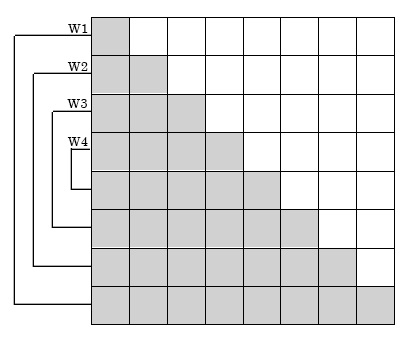
\includegraphics[width=0.55\textwidth]{images/chapter_3/aglomerativo_mpi}
			
			
			\caption{División de las filas utilizada en la estrategia desarrollada para el algoritmo Jerárquico Aglomerativo}
			\label{fig:aglomerativo}
		\end{figure}
		
		%\begin{figure}[!h]
		%	\centering
		%	
		%	
		%	\begin{subfigure}[t]{0.4\textwidth}
		%		\centering
		%		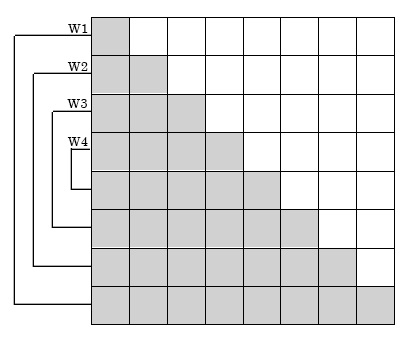
\includegraphics[width=\textwidth]{images/chapter_3/aglomerativo_mpi}
		%		\caption{División óptima}
		%		\label{fig:aglomerativompi}
		%	\end{subfigure}
		%	\hfill
		%	\begin{subfigure}[t]{0.52\textwidth}
		%		\centering
		%		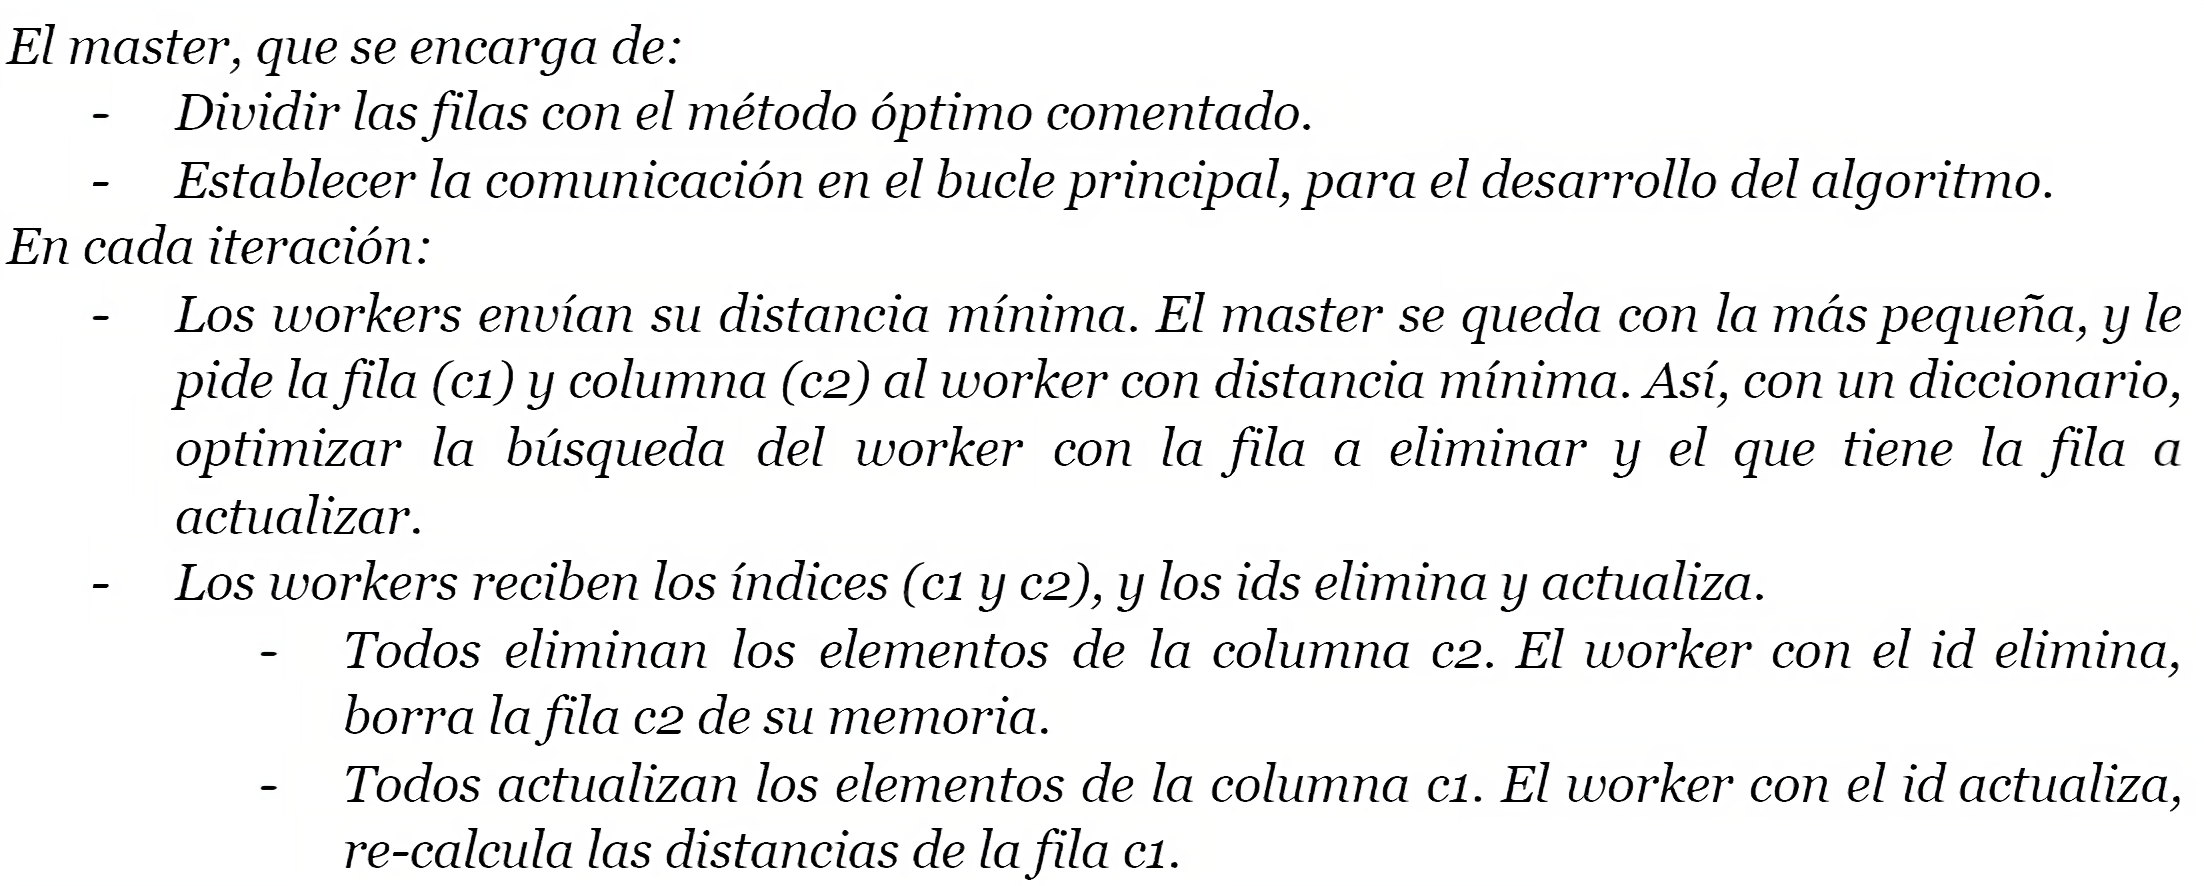
\includegraphics[width=\textwidth,height=5cm]{images/chapter_3/aglomerativo_sec}
		%		\caption{Tareas de los proceso}
		%		\label{fig:aglomerativosec}
		%	\end{subfigure}
		%	
		%	\caption{MPI - Jerarquico Aglomerativo}
		%	\label{fig:aglomerativo}
		%\end{figure}
		
		
		Una vez descrito el reparto del espacio entre los procesos, cada uno tiene que ejecutar el algoritmo en paralelo, sincronizándose cada cierto tiempo para actualizar valores. Refrescando la memoria, este algoritmo, en cada iteración, agrupa los dos individuos más cercanos, eliminando una fila y columna de la matriz. El bucle principal de la estrategia, se repite hasta que solo haya \textit{C} clusters. Las etapas son las siguientes:
		
		\begin{enumerate}
			\item El \textit{master} pide a los \textit{workers} la celda con menor valor (menor distancia entre los clusters \textit{i} y \textit{j}, siendo estos la fila y columna). 
			\item El \textit{master}, con los valores recibidos, pide la fila (\textit{i}) y la columna (\textit{j}) del \textit{worker} con menor distancia. Con estos datos, el \textit{master} envía a todos los procesos estos índices, así como los \textit{ids} de los \textit{workers} que tienen que eliminar o actualizar la fila con mayor o menor índice respectivamente.
			\item Todos los \textit{workers} eliminan la columna con mayor índice. El \textit{worker} que tiene que eliminar la fila la elimina. Mientras que el que tiene que actualizar la actualiza, con o sin ayuda de los demás \textit{workers}.
		\end{enumerate}
								
		
		El cálculo de las distancias de la nueva fila (actualización) usando la distancia centroide es lineal, no se puede reducir el tiempo de ejecución. Pero para los enlaces simples y completos, que tienen un coste cuadrático, se debe intentar reducir el tiempo de cómputo. Para lograrlo se generan otras dos estrategias más, que lo único que cambian de esta primera estrategia es como se divide el cálculo de la actualización de la fila entre todos los \textit{workers}. 
		
		El objetivo es encontrar una manera lo más optimizada posible de realizar el cálculo. 
		\begin{itemize}
			\item Cuando hay pocos individuos por \textit{cluster}, es más probable que haya muchas columnas que actualizar, y conviene dividir el cálculo de distancias de todas las celdas entre los procesos disponibles. 
			\item Sin embargo, cuando aumenta el número de individuos, se reducen las columnas y esta idea ya no resulta viable. Cada nueva distancia requiere de un cómputo significativo realizando los cálculos. Por eso, es mejor juntar a todos los procesos para calcular las distancias de forma escalonada, dividiendo los individuos del \textit{cluster} para encontrar la distancia mínima (simple) o máxima (completa).
		\end{itemize}
		
		La segunda estrategia se basa en esto, es por eso que el \textit{worker} con la fila a actualizar tiene en cuenta cuantos clusters tiene el algoritmo en el momento de la actualización. Si es mayor a la mitad, el cálculo de las nuevas distancias se reparte entre los procesos. En caso contrario, el \textit{worker} envía a todos los \textit{workers} disponibles la misma celda, para que se divida la búsqueda de la menor o mayor distancia.
		
		La tercera estrategia no tiene en cuenta esto, siempre se dividen las celdas de las nuevas distancias, pero esta vez añadiendo procesos extra que se encargan exclusivamente de realizar estos cálculos. Además de los procesos \textit{workers} que trabajan en el bucle principal del algoritmo.
		
		
	\subsection{K-Medias}
	\label{cap:3_2_2}
		De manera similar al algoritmo anterior, K-medias pertenece al aprendizaje no supervisado. Esta vez se aplica un valor \textit{K} sujeto a una asignación flexible según nuestros criterios. Al contrario que el algoritmo jerárquico aglomerativo, no se utiliza una matriz, y solo se usa distancia por centroides. Las estrategias para este algoritmo son las siguientes:		
		
		
		\begin{enumerate}
			\item Reparto estático. Dividir la población entre los \textit{workers}, como muestra la Figura \ref{fig:kmediasdiv}. 
			\item Reparto dinámico. En cada iteración del algoritmo, wl \textit{master} envia individuos a los \textit{workers}. Cuando finalicen el procesado, envían de vuelta la agrupación y esperen a recibir otros individuos. 
		\end{enumerate}
		
		La primera idea es la más simple y la que mejor suena en un primer momento. El \textit{master} se encarga de generar los centroides de manera aleatoria, eligiendo K individuos al azar, sin repeticiones. Mediante broadcast los \textit{workers} reciben estos centros, y con conexiones punto-a-punto se recibe la población dividida sin intersecciones. Cada \textit{worker} se encarga de una subpoblación. 
		
				
		\begin{mdframed}[roundcorner=5pt]
			El siguiente proceso se repite hasta que el \textit{master} envíe un mensaje de finalización, es decir, no cambien los centros:	
			\begin{itemize}
				\setlength\itemsep{0em} 
				\item Los \textit{workers} calculan la asignación de sus individuos. Además, calculan la suma de distancias de los individuos a sus centros y el número de individuos asociado a cada cluster. Estos valores los envían al \textit{master}.
				\item El \textit{master} recibe estos valores y calcula los nuevos centroides. Manda un mensaje a todos los \textit{workers}. 
				\begin{itemize}
					\setlength\itemsep{0em} 
					\item \textit{CentroidesNuevos}, si los centros cambian. Se actualizan los centros.
					\item Finalización, en caso contrario.
				\end{itemize}
			\end{itemize}
		\end{mdframed}
		
	
		
		Después de implementar la primera opción, reparto estático, no es una buena idea implementar un reparto dinámico. El constante flujo de mensajes aumenta el tiempo de ejecución y la población a categorizar no cambia, por lo que distribuir la población una única vez en toda la ejecución es más eficiente. Lo único que cambia en cada iteración es la asignación de los individuos, el algoritmo finaliza cuando la asignación no varíe entre iteraciones (centros de los clusters). El algoritmo se repite \textit{iter} veces, valor que depende de la asignación de los individuos y los centros de los clusters. Si además de parar la ejecución al recibir todos los individuos, se para de nuevo para reenviarlos al final de cada iteración, perdemos \textit{iter} veces más tiempo al enviar los individuos a los procesos \textit{workers}. 
		
		
		\begin{figure} [!h]
			\centering
			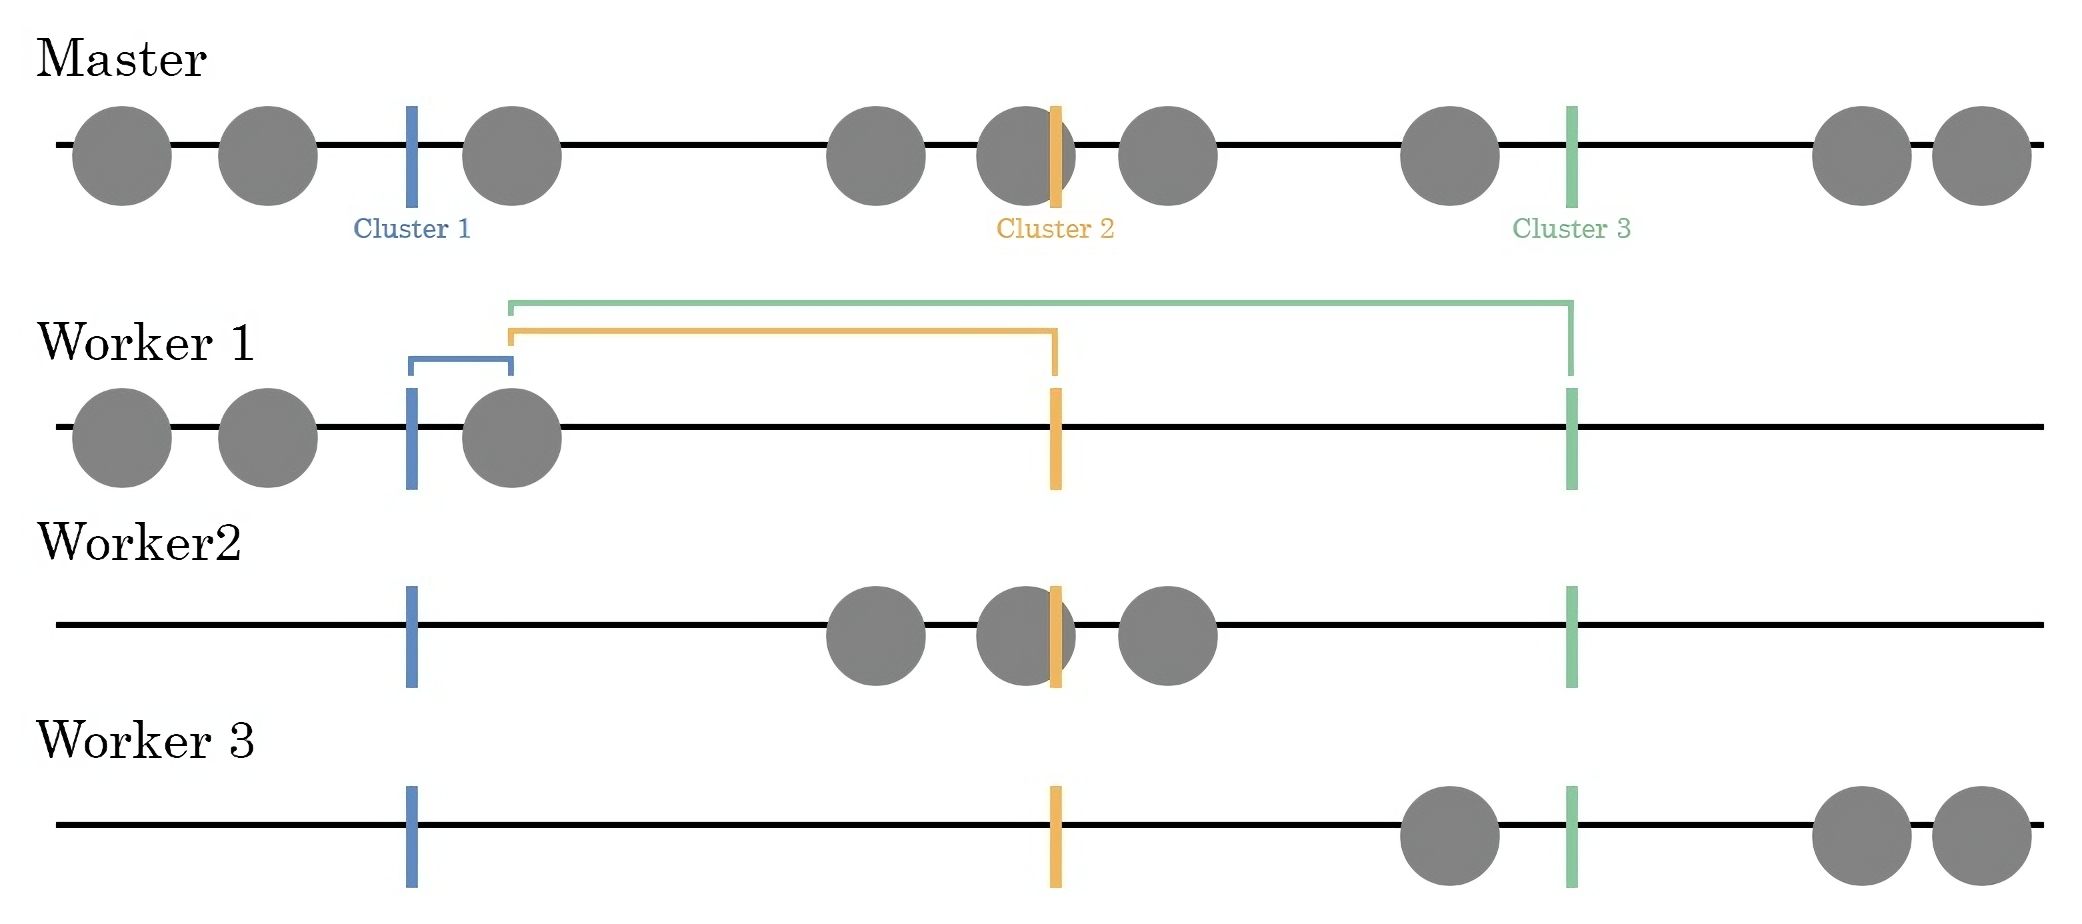
\includegraphics[width=0.8\textwidth]{images/chapter_3/kmedias_mpi}	
			\caption{División de las poblaciones entre los procesos \textit{workers} en la primera estrategia del algoritmo K-Medias}
			\label{fig:kmediasdiv}
		\end{figure}
		
		\newpage
		
		Como se comentó en el capítulo anterior, este algoritmo se tiene que repetir varias veces para encontrar la mejor asignacion, el óptimo general. A su vez, también hay que variar el valor de \textit{K} para buscar la mejor asignación para los individuos. Para lograr este objetivo se puede enfocar de dos diferentes formas:
		
		\begin{enumerate}
			\item Aplicar la implementación anterior con varios bucles. El externo para variar el valor de \textit{K} y el interior para repetir el algoritmo.
			\item Ejecutar en cada proceso \textit{worker} el algoritmo sin mejoras. Los \textit{workers} ejecutan la búsqueda con valores distintos de \textit{K} y el \textit{master} se encarga de almacenar los mejores resultados.
		\end{enumerate}
		
		Como muestra la Figura \ref{fig:KMedias_comp}, ambas ideas tienen el mismo coste temporal, sin contar el overhead (tiempo consumido para la comunicación de mensajes entre procesos). Pero, la segunda opción, al tener en cada proceso una copia de la población entera, tiene mayor complejidad espacial. Este aumento del uso de memoria para poblaciones elevadas, provoca que no se pueda ejecutar esta estrategia con muchos procesos. A no ser que el ordenador donde se ejecuta la estrategia tenga disponible mucha memoria libre.
		
		\begin{figure} [!h]
			\begin{mdframed}[roundcorner=5pt]
				\[
				O\left((T * \frac{N * K}{M}) * \text{Rep} * K_{\text{max}}\right) \approx O\left(\frac{{(T * (N * K)) * \text{Rep} * K_{\text{max}}}}{{M}}\right)
				\]
				
				
				
				\begin{tcolorbox}[boxrule=0.5pt, fontupper=\small]
					
					\textit{T} = número de iteraciones en el algoritmo de K-Medias\\
					\textit{N} = número de individuos en la población\\
					\textit{M} = número de procesos \textit{workers}\\
					\textit{K} = número de clusters\\
					\textit{Rep = }repeticiones para buscar el óptimo general\\
					\textit{K\(_{Max}\)} = valor máximo de K en la búsqueda.				
					
				\end{tcolorbox}
				
			\end{mdframed}
			\caption{Comparación temporal de las estrategias de búsqueda del óptimo general para el algoritmo de K-Medias}
			\label{fig:KMedias_comp}
		\end{figure}
		
		
		
		
	\subsection{K-Vecinos más cercanos (KNN)}
	\label{cap:3_2_3}
		Al contrario de los algoritmos anteriores, KNN (K-Nearest Neighbors en inglés) pertenece al aprendizaje supervisado, por lo que necesita una población ya categorizada para poder agrupar los nuevos individuos. Al igual que el algoritmo K-Medias, y como menciona su nombre, esta técnica de clustering utiliza una variable \textit{K}, que representa los vecinos que se van utilizar para categorizar los individuos.
		
		Aplicando una cola de prioridad de máximos para el cálculo de los \textit{K} vecinos más cercanos, reducimos la complejidad del algoritmo. Al recorrer la población categorizada, se compara con la cima de la cola. Si la distancia a comparar es menor que la cima, se elimina la cima y se introduce la nueva distancia. Los valores de la cola se mueven con la restricción de prioridad, y al finalizar la búsqueda en la población se cuentan los elementos de la cola para saber qué cluster se repite más.
		
		Es importante actualizar la población conforme se van prediciendo los valores, para tener más puntos de referencia. Si no actualizamos la población, la agrupación de los individuos puede variar de forma significativa. Aunque es menos precisa a la hora de predecir, el algoritmo es más veloz, al no aumentar la población categorizada no tiene que recorrer un individuo más conforme se categoriza la población a predecir. Al contar con una población extra (la categorizada) se proponen dos estrategias posibles:
		
		
		\begin{enumerate}
			\item Dividir la población categorizada entre los \textit{workers} (ver Figura \ref{fig:knn1})
			\item Dividir la población a predecir entre los \textit{workers} (ver Figura \ref{fig:knn2})
		\end{enumerate}
		
		Si dividimos la población categorizada (primera estrategia), los \textit{workers} cuentan con menos cómputo en cada individuo. Comparan el individuo a predecir con su subpoblación, y el \textit{master} tiene una mayor carga de trabajo, al recibir los \textit{K} vecinos de cada \textit{worker} y tener que ver los \textit{K} mejores de todos los individuos recibidos.  Mientras que el \textit{master} comprueba las distancias recibidas, los \textit{workers} operan en la siguiente iteración, enfocándose en el próximo individuo a predecir. Si se actualizan los individuos, el \textit{master} reparte de forma equitativa los individuos que se categorizan. En cada iteración envía el individuo categorizado a uno distinto, utilizando un contador con el \textit{id} del \textit{worker} respectivo y aplicando la operación módulo con el número de \textit{workers} ejecutados.
		
		Con la división de la población a predecir (segunda estrategia), cada \textit{worker} realiza un cómputo equitativo, pero predicen menos individuos. El \textit{master} no realiza tantas tareas como en la estrategia anterior, solo recibe la categorización de los \textit{workers}. El proceso de actualizar la población se puede realizar de varias formas, ya que todos los \textit{workers} comparten la población categorizada. Una posible solución consiste en enviar \textit{M} nuevos individuos a los \textit{M} \textit{workers} ejecutados en cada iteración, es decir, al recibir un individuo predicho de cada \textit{worker}. O cada \textit{X} iteraciones, enviar los nuevos individuos categorizados.
		
		\vspace{-0.25cm}
		\begin{flushleft}
			El coste espacial depende de los tamaños de las poblaciones.		
		\end{flushleft}
		\vspace{-0.75cm}
		
		\begin{itemize}
			\item La primera estrategia, al dividir la población inicial, es más eficiente cuando esta población inicial es mayor que la población de predicción. 
			\item En su contraparte, en la segunda estrategia, al dividir la población a predecir, tiene un mejor rendimiento con poblaciones de predicción mayores.
		\end{itemize}
		
		\begin{figure}[!h]
			\centering
			
			
			\begin{subfigure}[t]{0.45\textwidth}
				\centering
				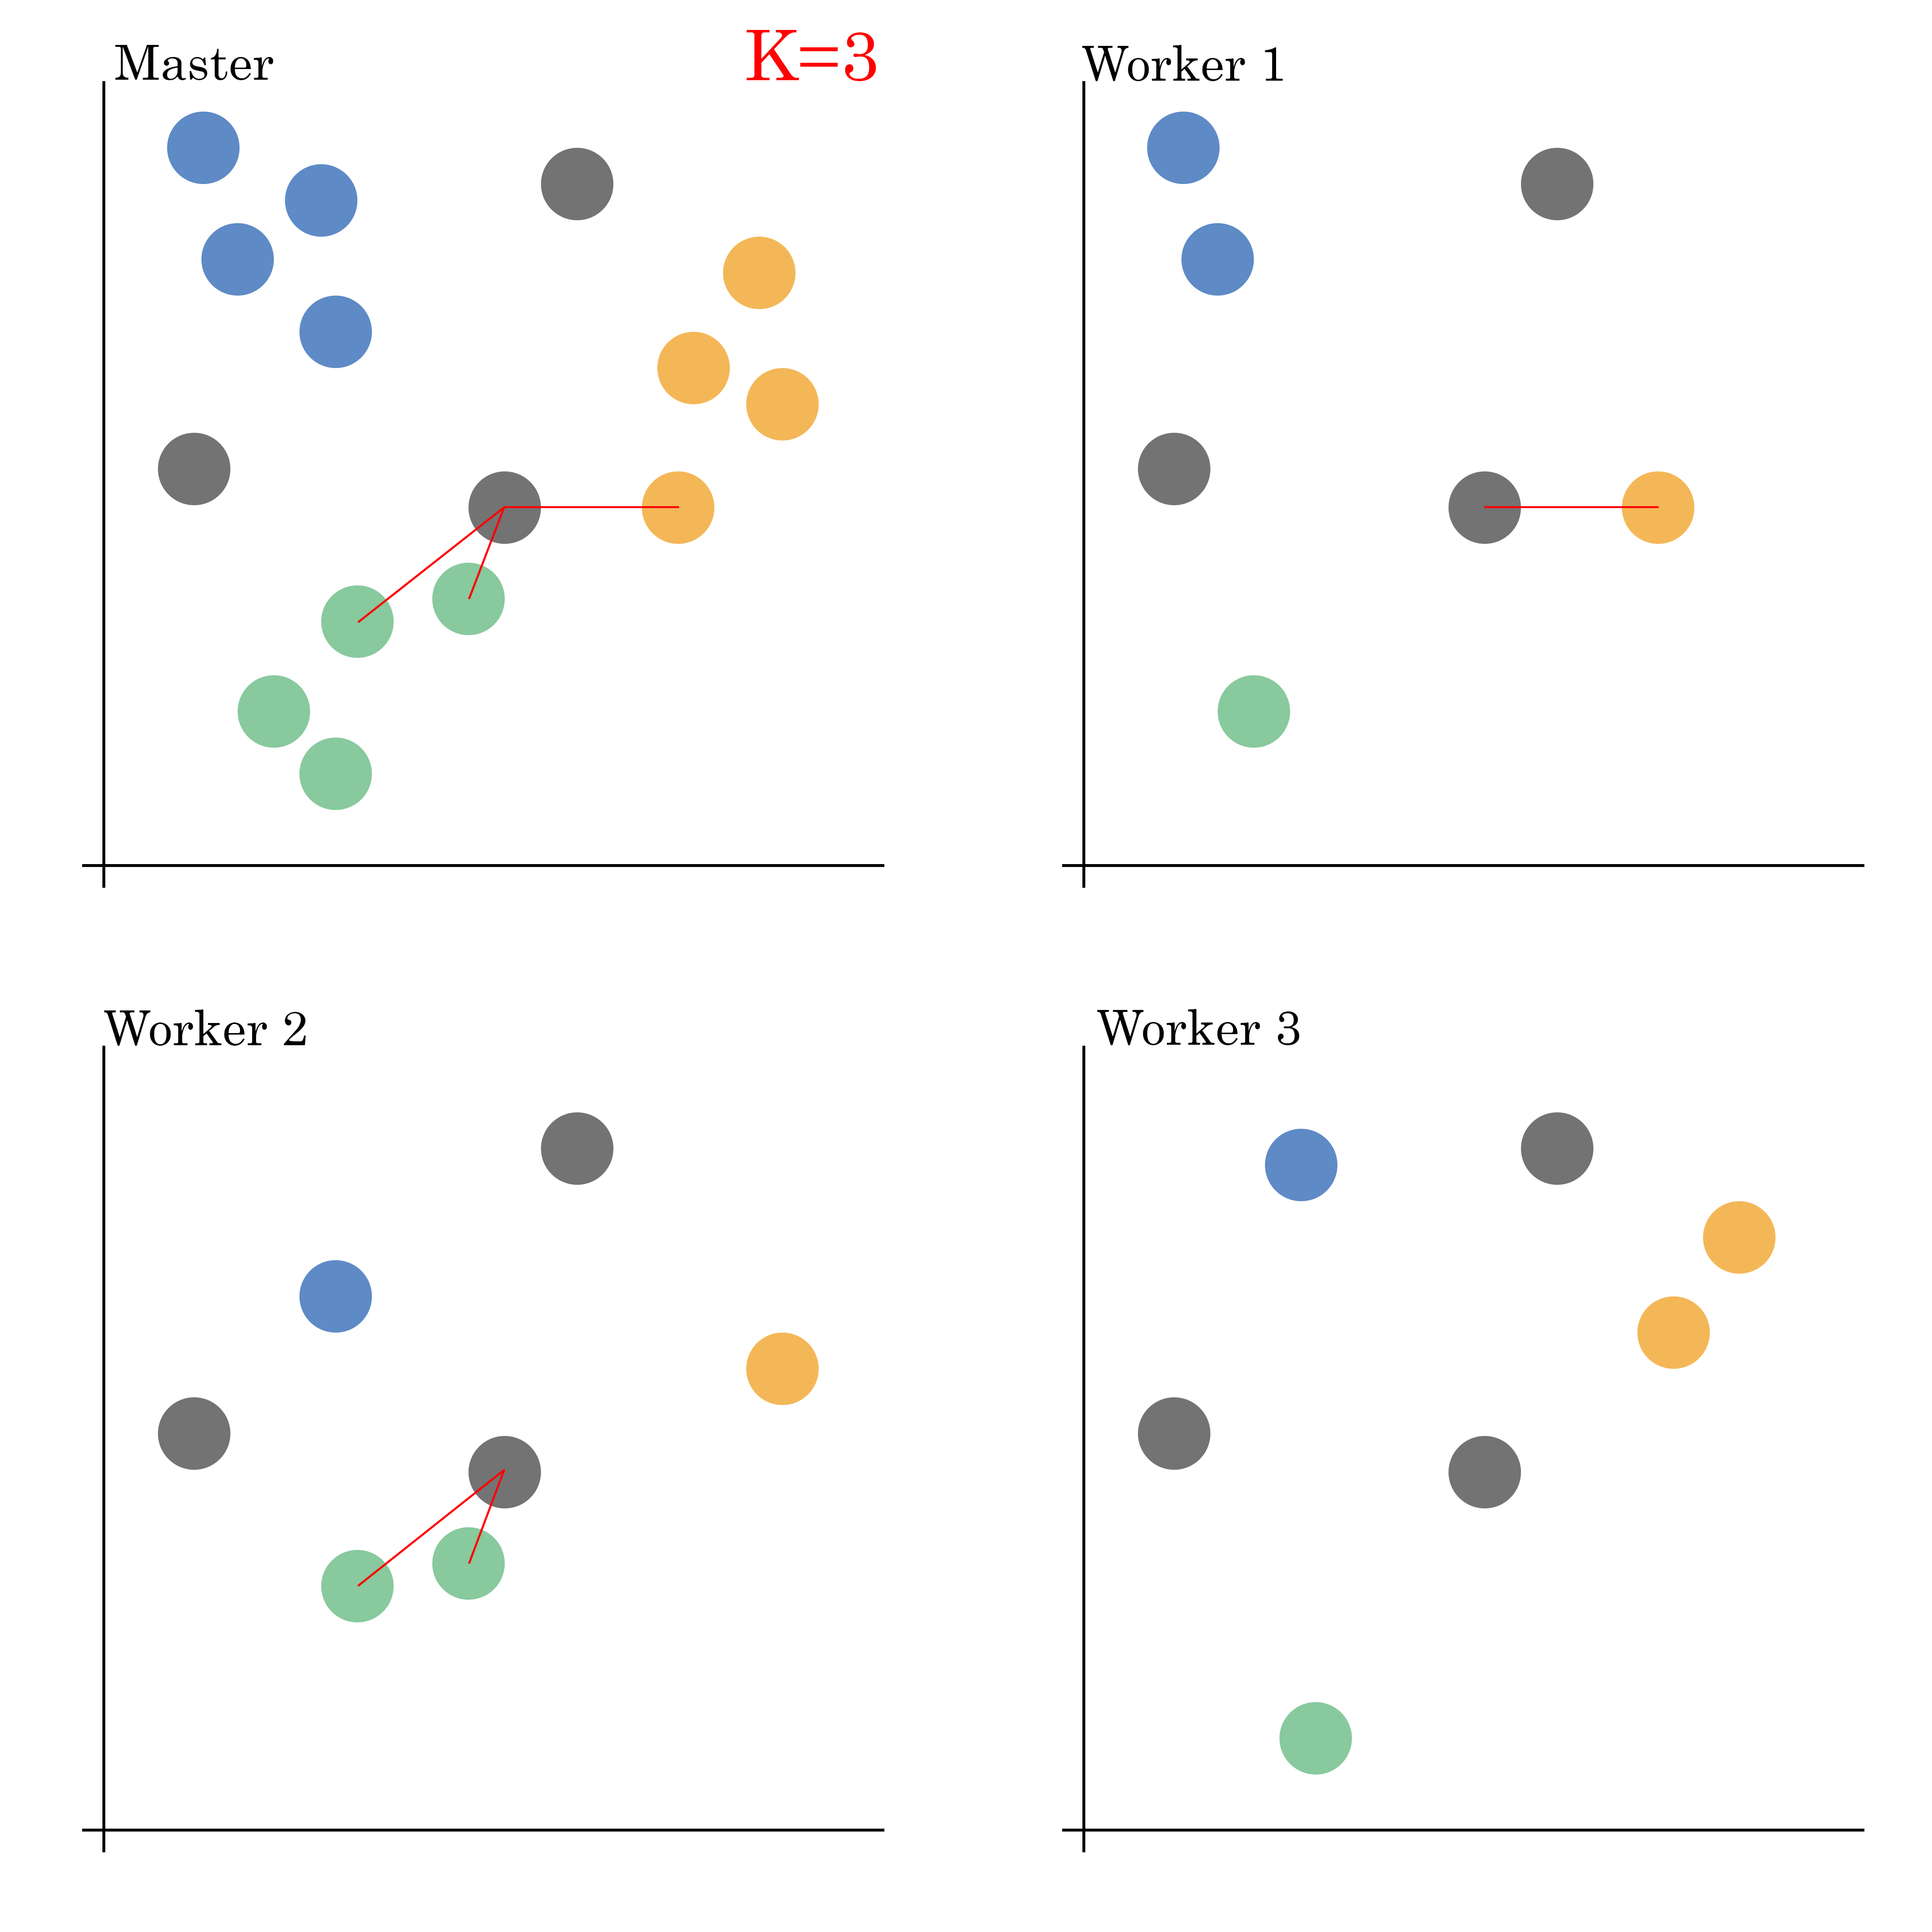
\includegraphics[width=\textwidth]{images/chapter_3/knn_mpi1}
				\caption{División de la población categorizada}
				\label{fig:knn1}
			\end{subfigure}
			\hfill
			\begin{subfigure}[t]{0.45\textwidth}
				\centering
				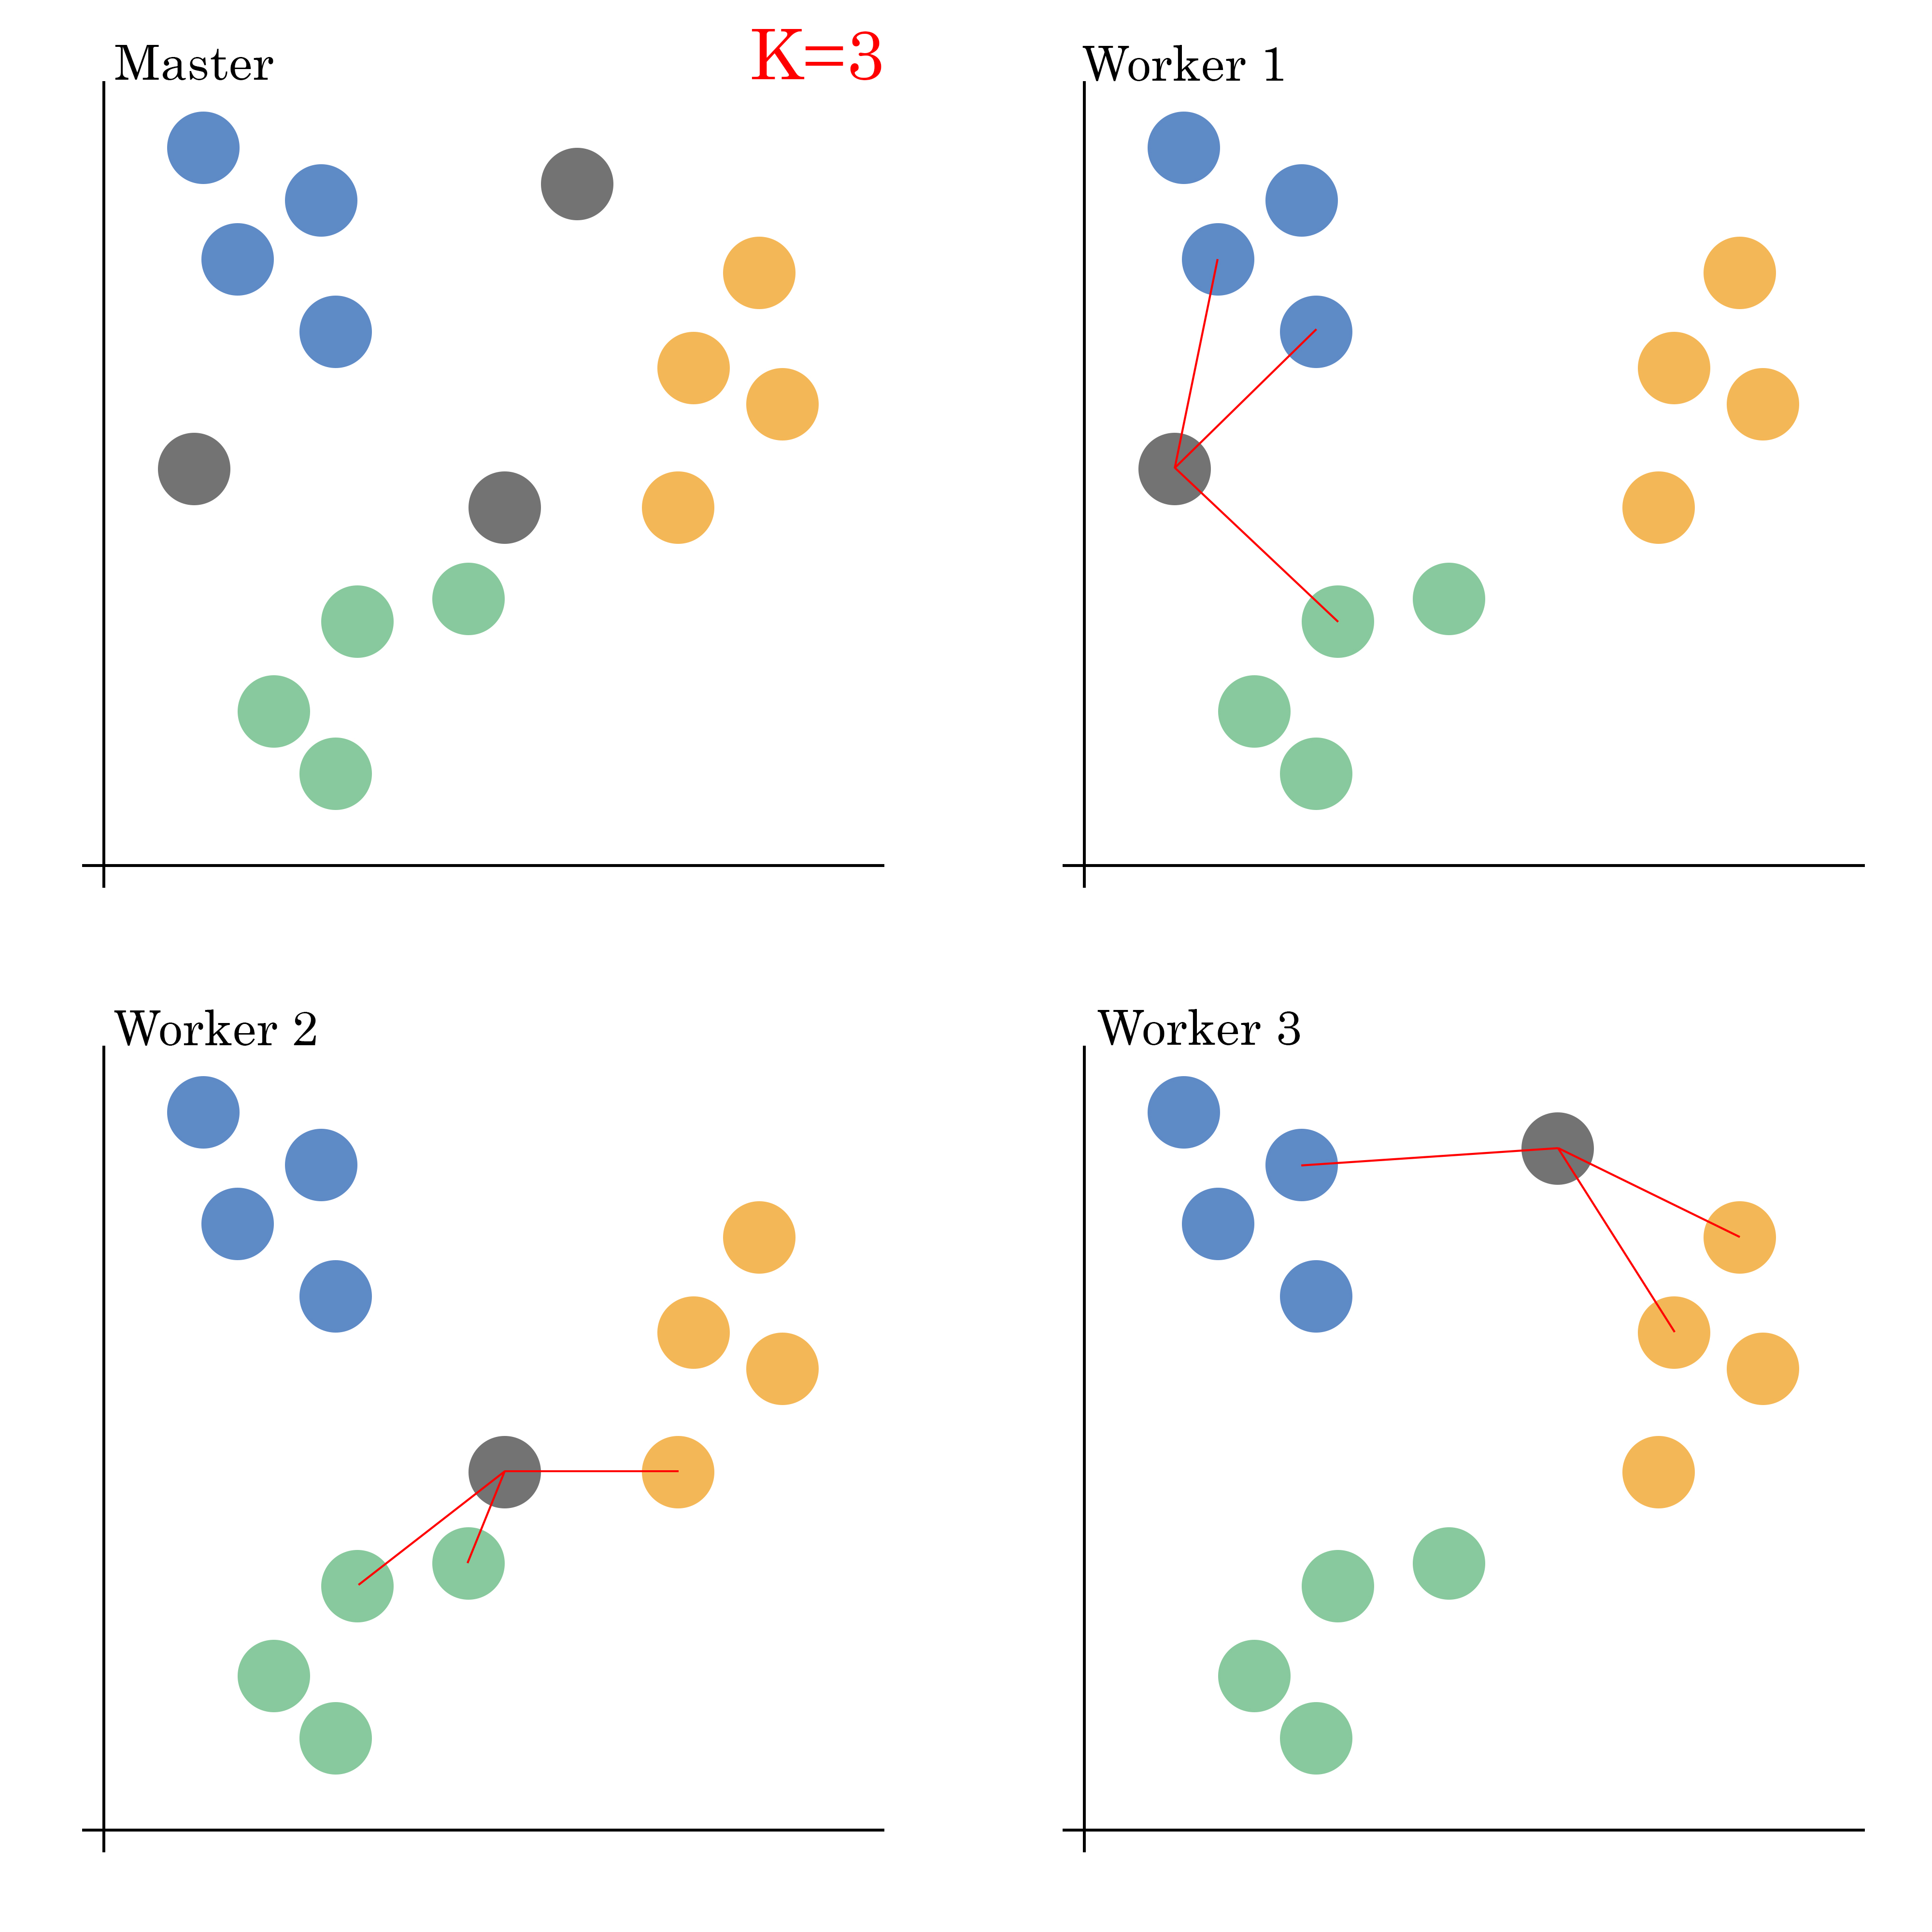
\includegraphics[width=\textwidth]{images/chapter_3/knn_mpi2}
				\caption{División de la población a predecir}
				\label{fig:knn2}
			\end{subfigure}
			
			\caption{Estrategias para paralelizar el algoritmo KNN}
			\label{fig:knnmpi}
		\end{figure}

		El proceso \textit{master} (el de la esquina superior izquierda en ambas figuras) tiene el dataset completo. En la primera estrategia (gráfico de la izquierda) divide la población categorizada (individuos representados con colores) entre los procesos y mantiene una copia en todos los procesos de la población a predecir (individuos representados en gris). La segunda estrategia (gráfico de la derecha) tiene una copia de la población categorizada en todos los procesos y una subpoblación de la población a predecir.
		
		
		En este algoritmo también hay que realizar una búsqueda del mejor valor para \textit{K}. Sin embargo, al contrario que en K-Medias, no hace falta repetir varias veces el mismo algoritmo, ya que el proceso es determinista. Es decir, con la misma población, siempre se obtiene la misma predicción. Aunque puede llegar a cambiar dependiendo del orden de categorización de la población a predecir. 
		
		No hay que repetir el mismo algoritmo varias veces, pero puede llegar a ser útil variar el número de vecinos (valor de \textit{K}). Las mejoras de esta búsqueda son las mismas que en el algoritmo anterior: 
		
		\begin{enumerate}
			\item Aplicar alguna de las dos implementaciones comentadas anteriormente, con un bucle que varíe la variable \textit{K}. 
			\item Ejecutar en cada proceso \textit{worker} el algoritmo sin mejoras. El \textit{master} se encarga de almacenar los mejores resultados.
		\end{enumerate}
		
		


\section{Aprendizaje por refuerzo}
	\label{cap:3_3}
	Los algoritmos de este tipo de aprendizaje actualizan iterativamente las estimaciones de calidad de las acciones permitidas en el entorno de desarrollo, y pueden ser almacenados en una tabla o aplicar una red neuronal.
	
	\subsection{Q-Learning}
	\label{cap:3_3_1}
		El algoritmo Q-Learning, es el más básico del aprendizaje por refuerzo. Las estimaciones de las mejores acciones para cada estado se almacenan en una Q-Table representada como una matriz en la que cada fila es un estado, y las columnas son las acciones disponibles. 
		
		Este algoritmo tiene numerosas aplicaciones. Nos centramos en la técnica de minimizar las acciones, para llegar desde una celda origen a un destino. El laberinto tiene un tamaño y semilla variable por parámetros de inicialización. Para lograr su objetivo dispone de acciones de movimiento en los dos ejes cardinales, norte, sur, este y oeste. No puede atravesar ni situarse en un muro del laberinto, y para que el agente aprenda a moverse por el laberinto y llegar a la meta hay que fijar unas recompensas:
		\begin{itemize}
			\item Si se choca con un muro castigamos al agente con valores altos para que no añada movimientos innecesarios para alcanzar su objetivo.
			\vspace*{-0.2cm}
			\item Al moverse, el agente recibe un castigo pequeño para que aprenda a minimizar las operaciones.
			\vspace*{-0.2cm}
			\item Al llegar a la meta le damos una recompensa alta, para que aprenda a la celda destino. 					
		\end{itemize}
	
		Con estas recompensas, el agente aprende a llegar a la meta minimizando las acciones ejecutadas. El código que genera los laberintos ha sido implementado por @ChlouisPy en github\cite{MazeGenerator}


		Antes de enfocarnos en las implementaciones MPI, hay que comentar una mejora que se puede aplicar a el algoritmo básico de Q-Learning. Realizar un preprocesado. Modificar la Q-Table, convertiéndola en un array bidimensional, en el cual no se almacenen las acciones que no deseamos que realice el agente, como puede ser chocarse con un muro. O eliminar estados innacesibles como situarse en un muro.
		
		Esta mejora puede reducir el tiempo de cómputo, al no perder tiempo realizando acciones innecesarias para alcanzar su objetivo. Además de reducir la complejidad espacial, al reducir el número de estados. Un desventaja es que añade otras estructura adicional (array bidimensional) para almacenar las acciones para cada estado. 
		
		Este preprocesado tiene complejidad cuadrática \textit{O(4*N\(^{2}\)) $\equiv$ O(N\(^{2}\))}, siendo \textit{N} el número de filas y columnas. Recorre toda la matriz, comprobando para cada celda si no es un muro, y en caso afirmativo itera en las cuatro direcciones permitidas para almacenar las acciones disponibles para la celda actual (estado). Con tamaños de laberintos pequeños no hace falta paralelizar el preprocesado, porque no se consigue reducir el tiempo significativamente. Laberintos con más de mil filas y columnas si se consigue reducir el tiempo de cómputo.
		
		
			
		En los algoritmos del bloque anterior se necesitaba realizar una búsqueda para encontrar el óptimo general. En este algoritmo conviene realizar otra búsqueda, pero esta vez para encontrar combinaciones de los hiper-parámetros ($\alpha$, $\gamma$, $\epsilon$). Son muy importantes para el desarrollo del agente en el entorno. Una mala configuración de éstos hace que sobre aprenda -o no aprenda- correctamente, generando bucles infinitos. Por este motivo es importante comprobar las diferentes combinaciones de hiper parámetros, y comprobar, cuales funcionan correctamente en el entorno. La búsqueda en laberintos grandes es muy lenta, ya que hay que comprobar muchas combinaciones entre los hiper-parámetros y los episodios del entrenamiento. Por eso es más útil desarrollar el algoritmo Deep Q-Learning que no tiene problemas con los estados, al usar una red neuronal. Pero si queremos usar el algoritmo básico de Q-Learning, hay que realizar una búsqueda exhaustiva en el entorno ejecutando una cantidad significativa de combinaciones de hiper parámetros.

		Para paralelizar esta búsqueda se ejecuta el algoritmo básico con el preprocesado mencionado en cada proceso \textit{worker}. Hay que desarrollar una estrategia para que cada \textit{worker} reciba una combinación de parámetros distinta, y así no haya repeticiones, perdiendo tiempo de cómputo. El \textit{master} se encarga de repartir combinaciones de hiper-parámetros. Con una precisión previamente inicializada, el \textit{master} aumenta un hiper-parámetro hasta llegar al \textit{100\%}. Cuando llega a dicho límite, se reinicia la variable y se aumenta la siguiente. Este proceso continua hasta llegar al \textit{100\%} de todos los hiper-parámetros. Cada \textit{worker} se encarga de una combinación recibida. Cuando termina el algoritmo, ya sea por bucle infinito o finalización correcta, envía un mensaje al \textit{master} con la información de finalización y los hiper-parámetros usados.
		
		Si el mensaje de finalización indica ``bucle'', el proceso ha terminado para evitar que se convierta en un proceso inactivo, pues dicha conbinación no converge hacia el objetivo. Estos bucles se detectan en el entrenamiento o la evaluación. Hay un bucle en el entrenamiento si un episodio tarda más de \textit{X} segundos en finalizar. En la evaluación se comprueba teniendo en cuenta los últimos cuatro estados visitados. Pues avanza y retrocede constantemente. 
		\begin{center}
			\textit{Estados[0]==Estados[2] and Estados[1]==Estados[3] and Estados[0]!=Estados[1]: }
		\end{center}
		
		

		Una vez realizada una búsqueda de las combinaciones de hiper-parámetros eficaces, se pueden emplearse para las siguientes mejoreas:
		
		\begin{enumerate}
			\item Dividir el entorno (laberinto) entre los procesos.
			\item Ejecutar el algoritmo en los \textit{workers} y juntar las experiencias.
		\end{enumerate}

	
		
		Al dividir el laberinto entre los procesos (primera mejora), cada proceso controla una zona, y se genera un flujo constante de episodios (iteraciones del algoritmo). Cuando un agente sale del dominio de un proceso, este le manda un mensaje al proceso que controla esa parte del laberinto con la posición en la que entra. La Figura \ref{fig:rlmpi} muestra como se divide un posible laberinto entre los procesos. Además de mostrar tres episodios con sus respectivos agentes (circulo en rojo). El \textit{master} se encarga de iniciar a los agentes en la celda en verde y cuando sale de su dominio envia al respectivo proceso y genera otro agente. 
		
		Para garantizar el correcto funcionamiento, el \textit{master} no puede recibir agentes de los \textit{workers}, en caso contrario no se podría garantizar el flujo de nuevos episodios. En la ejecución, solo puede existir \textit{M} agentes en todos los procesos (siendo \textit{M} el número de procesos ejecutados), debido a que un proceso solo puede gestionar a lo sumo un agente. Cada proceso tiene su propio dominio, lo que provoca que la Q-Table se divida entre éstos. Aplicando el preprocesado comentado anteriormente se dividen los dos arrays bidimensionales (acciones y Q-valores). 
		
		
		
		\begin{figure}[!h]
			\centering
			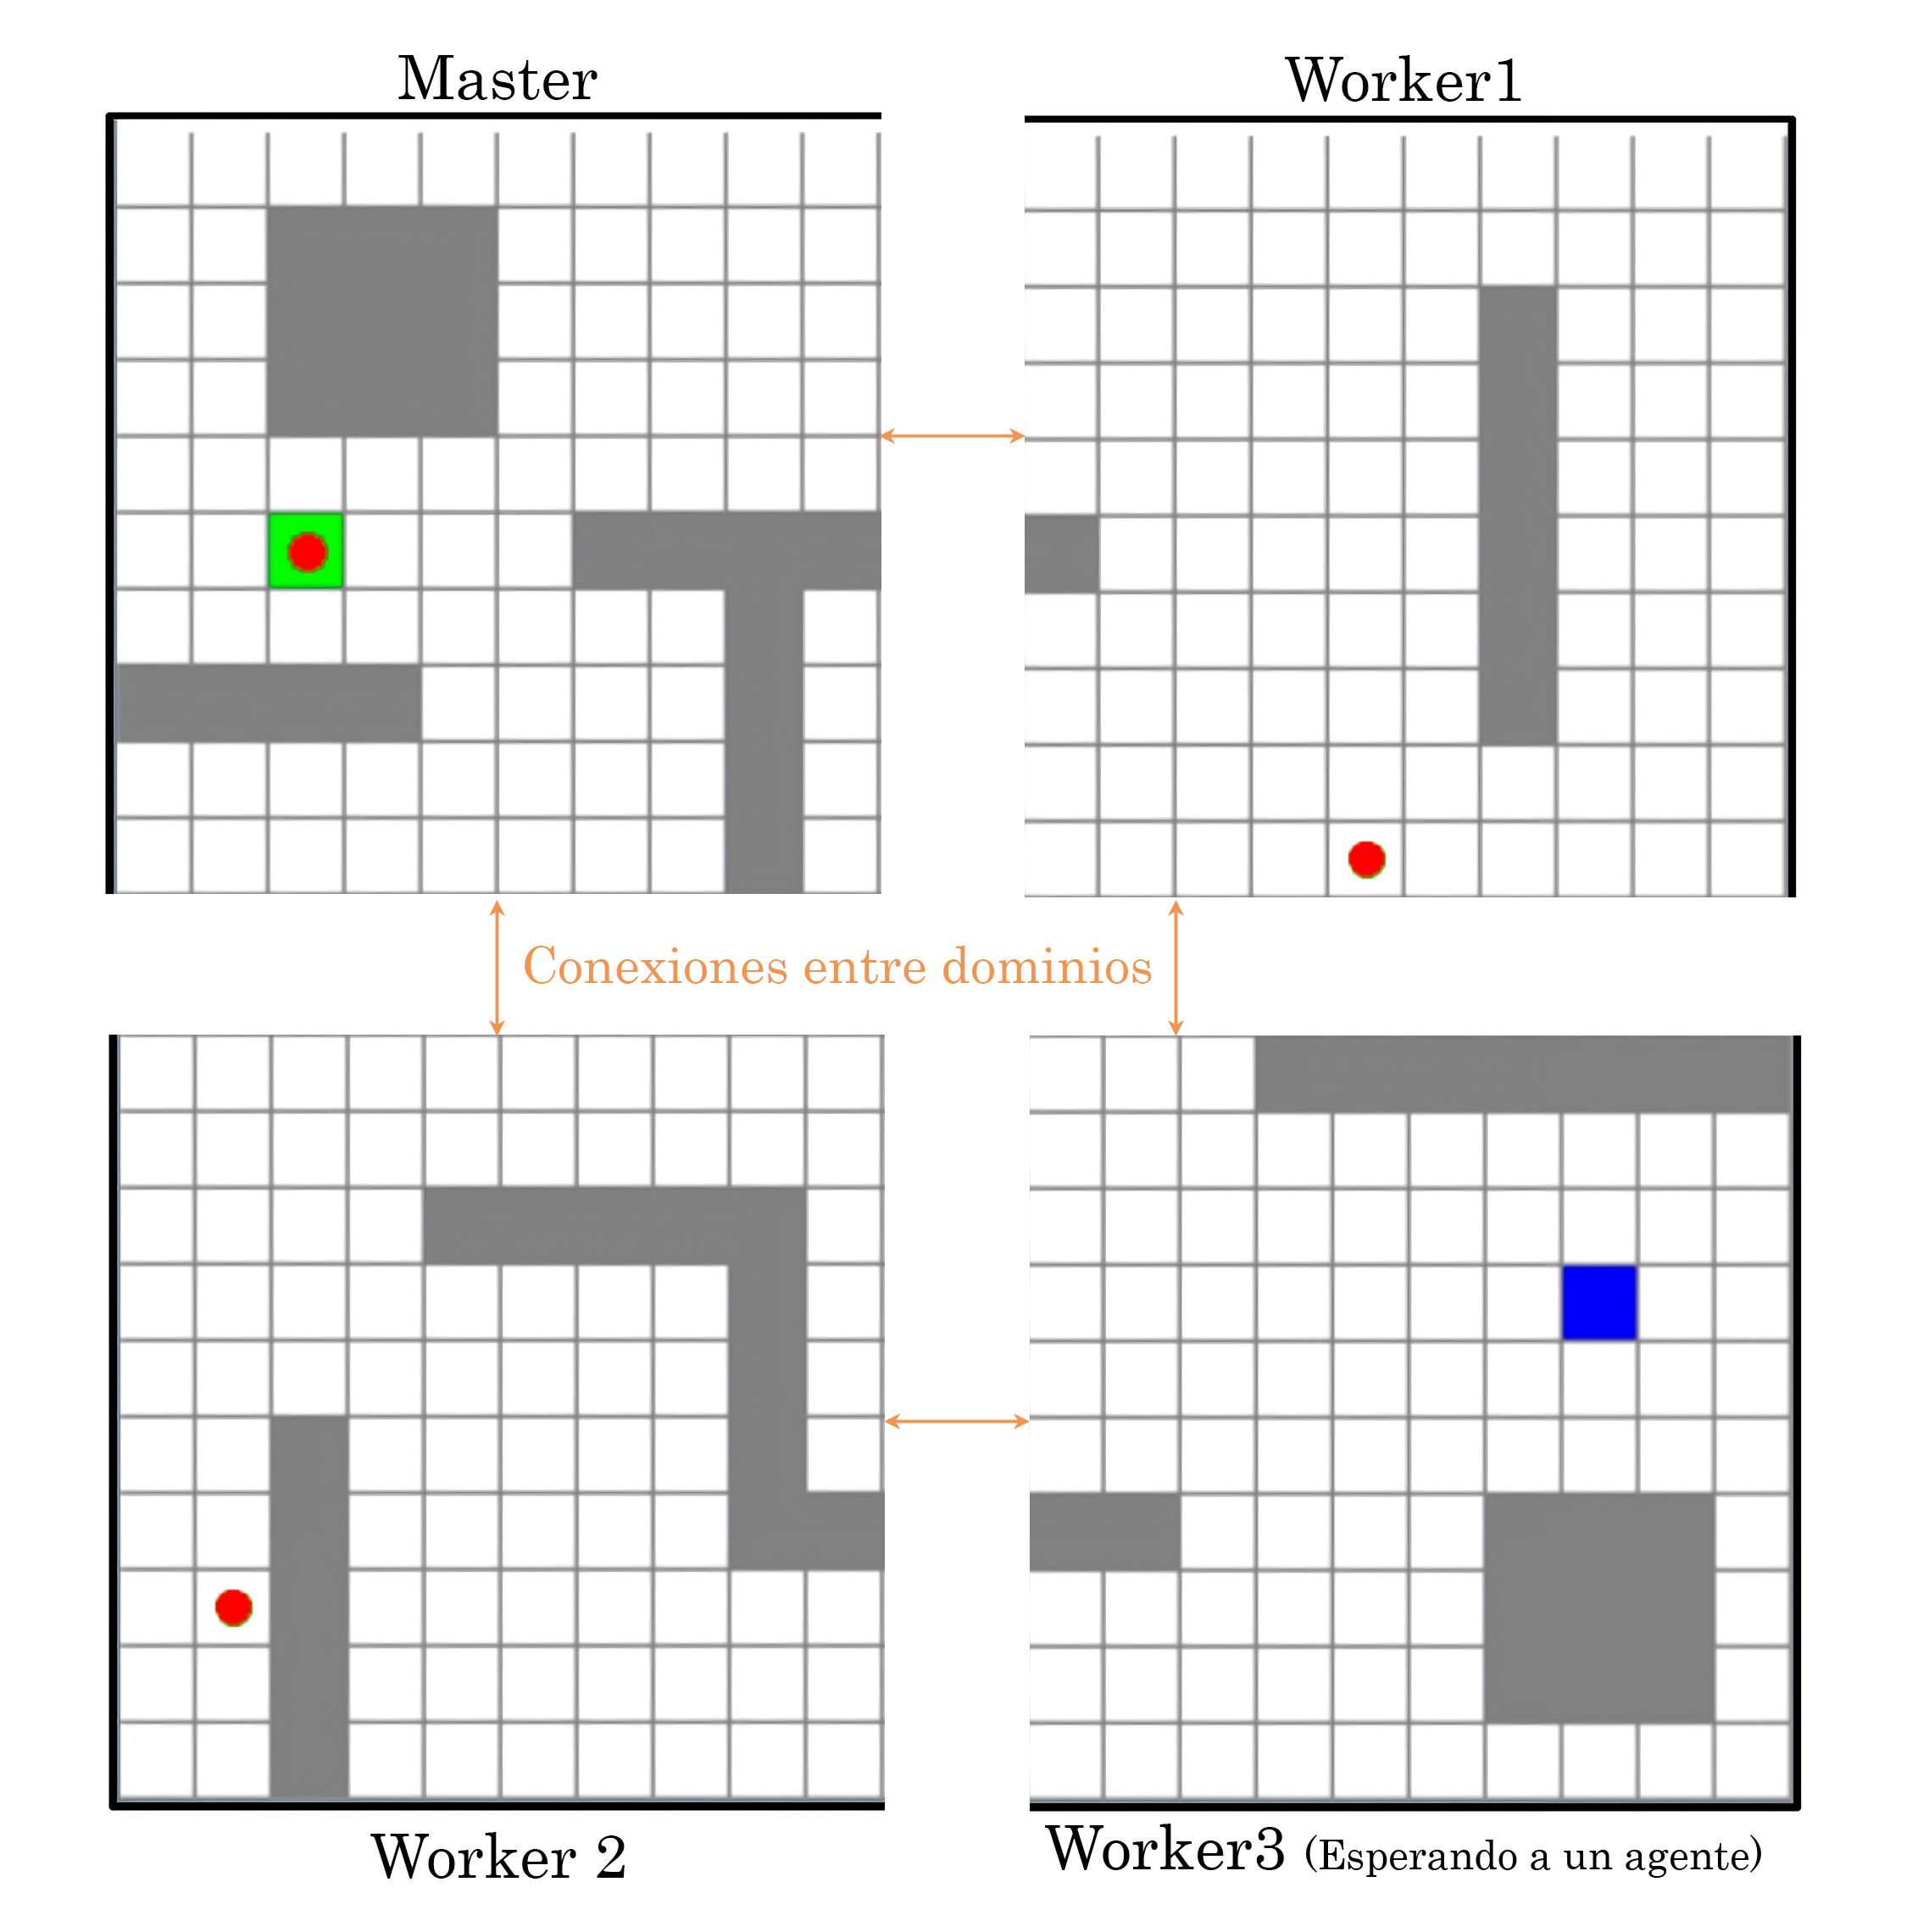
\includegraphics[width=0.6\textwidth]{images/chapter_3/rl_mpi}	
			\caption{División del entorno de la primera estrategia del agloritmo de Aprendizaje por Refuerzo}
			\label{fig:rlmpi}
		\end{figure}
	
		Aplicando la estrategia realizada en la búsqueda de hiper-parámetros, de ejecutar el algoritmo en varios procesos, se puede obtener la segunda estrategia. El \textit{master} recolecta las experiencias de los \textit{workers}, haciendo la media de los valor-Q obtenidos de los procesos, calculando así las mejores acciones para cada estado. Hay que tener en cuenta la posición de inicialización de los agentes en los procesos ejecutados. Si todos los procesos comparten el mismo punto de salida, los resultados serán parecidos a ejecutar el algoritmo en un solo proceso. Sin embargo al cambiar el punto de origen, los Q-valores obtenidos al realizar las medias de las experiencias varían y se recorre más espacio en menos tiempo. Y para lograr buenos resultados se asegura que al menos un proceso empieza desde el punto origen, de otra forma no se podría garantizar que el agente haya aprendido a alcanzar el destino desde la celda origen.			
			
			
	
	
	
	
	\subsection{Deep Q-Network}
	\label{cap:3_3_2}
		Este algoritmo utiliza redes neuronales para obtener la mejor acción para un determinado estado, eliminando así los problemas que tiene el algoritmo anterior. Con este método podemos abarcar entornos más complejos, y por eso se propone el juego de \textit{Namco} Pac-Man, cuya implementación  creamos desde cero para moldear a nuestro gusto la dificultad del entorno, así como facilitar el aprendizaje de la red neuronal. Nos centramos en obtener el mayor número de monedas antes de provocar una condición de finalización (ser comido por un fantasma o recoger todas los puntos). Para simplificar el entorno, no se desarrollan niveles en la ejecución, al igual de limitar la vida del agente a un único corazón, por lo que si es comido una única vez se termina la ejecución. Antes de profundizar en el algoritmo de IA, explicamos como funciona y hemos realizado la implementación del entorno.
	
		\begin{itemize}		
			\item Acciones disponibles. Como en el algoritmo anterior, son de movimiento. El agente y los fantasmas no pueden atravesar muros.
			\vspace*{-0.2cm}
			\item Entorno. Laberinto con muros, del cual no se puede escapar.
			\item Objetos del juego. 
			\vspace*{-0.3cm}
				\subitem - Pac-Man: el agente que mueve el usuario. Su objetivo es comer todos los puntos.
				\vspace{-1cm}
				\subitem - Fantasmas: se mueven siguiendo unos objetivos en el laberinto.
				\vspace{-0.2cm}
				\subitem - Túneles: puntos que se conectan de manera toroidal para no salir del entorno.
				\vspace{-0.2cm}
				\subitem - Puntos (pellets en ingles): son las "monedas" que el agente tiene que recoger.
				\vspace{-0.2cm}
				\subitem - Puntos de energia (powers): si el agente consume uno, durante un periodo de \hspace*{1.25cm} tiempo es invencible y puede comer a los fantasmas.				
				\vspace{-0.2cm}
				\subitem - Laberinto: entorno por el cual el agente y fantasmas se mueven.
			\vspace*{-0.3cm}
			\item Condiciones de finalización. Ganar obteniendo todas las monedas del laberinto o perder si un fantasma come al agente. 			
		\end{itemize}
		
		
		Los fantasmas tienen una IA interesante, pues tienen sus propios estados y cada uno tiene unos puntos objetivos que siguen para intentar comer al agente. Cabe recalcar que estos puntos están estratégicamente colocados para que los fantasmas trabajen en conjunto para cerrar huecos y poder atrapar al agente. El movimiento para alcanzar los puntos objetivos es simple, cuando se encuentran en una intersección (punto en el mapa con un hueco a la izquierda o derecha con respecto a su dirección actual) eligen la celda que minimice la distancia con respecto al punto objetivo. Los estados de los fantasmas son los cuatro siguientes:
		
		%\vspace{-0.9cm}
		\begin{itemize}
			\item Chase. Cada fantasma sigue unos puntos en movimiento.
			\vspace*{-0.3cm}
			\item Scatter. Sigue un punto estático fuera del laberinto para dar vueltas en una determinada zona.
			\vspace*{-0.3cm}
			\item Frightened. El agente puede comerlos, se mueve de manera aleatoria al llegar a una intersección.
			\vspace*{-0.3cm}
			\item Eaten. Han sido comidos y se encuentran en su casa esperando a salir. (Implementado de forma que espera \textit{3} movimientos del agente para salir)
		\end{itemize} 
		
		Los estados iteran con una secuencia principal \textit{[Scatter, Chase]}. La ejecución empieza con \textit{Scatter} para que los fantasmas, al salir de su casa, se dirijan a sus zonas asignadas. Al ejecutar, el agente, treinta acciones, el estado cambia a \textit{Chase} y se mantiene así sesenta acciones y vuelven a repetir la secuencia. Si el agente come un punto de energía, los fantasmas interrumpen su estado actual para pasar al estado \textit{Frightened} en el que están treinta acciones siendo vulnerables. Si el agente colisiona con un fantasma en este estado, es comido, pasando al estado \textit{Eaten}. Al finalizar este estado vuelven al inicio de la secuencia principal.
		
		\newpage
		
		\begin{flushleft}
			En la estado \textit{Chase} los fantasmas se mueven de la siguiente forma:
		\end{flushleft}
		
		\vspace{-0.9cm}
		\begin{itemize}
			\item Blinky (Rojo): Persigue directamente al agente.
			\vspace*{-0.3cm}
			\item Pinky (Rosa): Persigue la celda cuatro posiciones adelantada a donde apunta el agente. Si el agente mira hacia arriba, también añade cuatro celdas hacia la izquierda.
			\vspace*{-0.3cm}
			\item Inky (Azul): Persigue una celda en concreto que se calcula de la siguiente forma. Primero se calcula una posición como lo hace el fantasma rosa pero en vez de cuatro celdas, se hace con dos. El objetivo se calcula al añadir el vector de distancia de la posición del fantasma rojo a esta posición.
			\vspace*{-0.3cm}
			\item Clyde (Naranja): Si está a ocho o más celdas de distancia del agente, lo persigue. En caso contrario sigue su objetivo del estado Scatter.
		\end{itemize}
		
		
		El laberinto (mapa del entorno) se almacena en un fichero de texto, para representar las celdas vacías, muros, puntos o puntos de poder con números enteros (0, 1, 2 y 3 respectivamente).
		
		
		Al igual que en el algoritmo \textit{Q-Learning} la fase de entrenamiento es crucial, pues modifican los valores de la red neuronal para que el agente tome las mejores decisiones en cada estado, y terminar la ejecución sin perder. El entrenamiento se puede realizar de varias formas.	
			
							
		Si mantenemos el mismo estado inicial, el agente empieza siempre en el mismo punto, y depende mucho de los hiper-parámetros, además de la aleatoriedad. El agente empieza a investigar el entorno de manera aleatoria, y es muy probable que los fantasmas alcancen al agente bastante rápido sin explorar en profundidad el entorno. Por eso es mejor añadir varios estados iniciales para que pueda investigar el entorno de manera más eficiente. Hay que tener en cuenta que los estados iniciales tienen que ser puntos accesibles desde el estado inicial original. El agente no puede saltar a otras celdas sin coger los puntos del laberinto. La Figura \ref{fig:pacman_states} muestra un estado accesible y otro inaccesible con la misma posición del agente. El estado accesible ha recogido los puntos del laberinto, así como posicionado correctamente los fantasmas, en su contraparte el estado innacesible no ha recogido los puntos simulando una acción de salto por parte del agente. Si entrenamos con puntos aleatorios sin cambiar el estado del entorno, este entrenamiento no habrá surtido efecto, pues son estados que el agente no va a alcanzar nunca.
			
		
		\begin{figure}[!h]
			\centering
			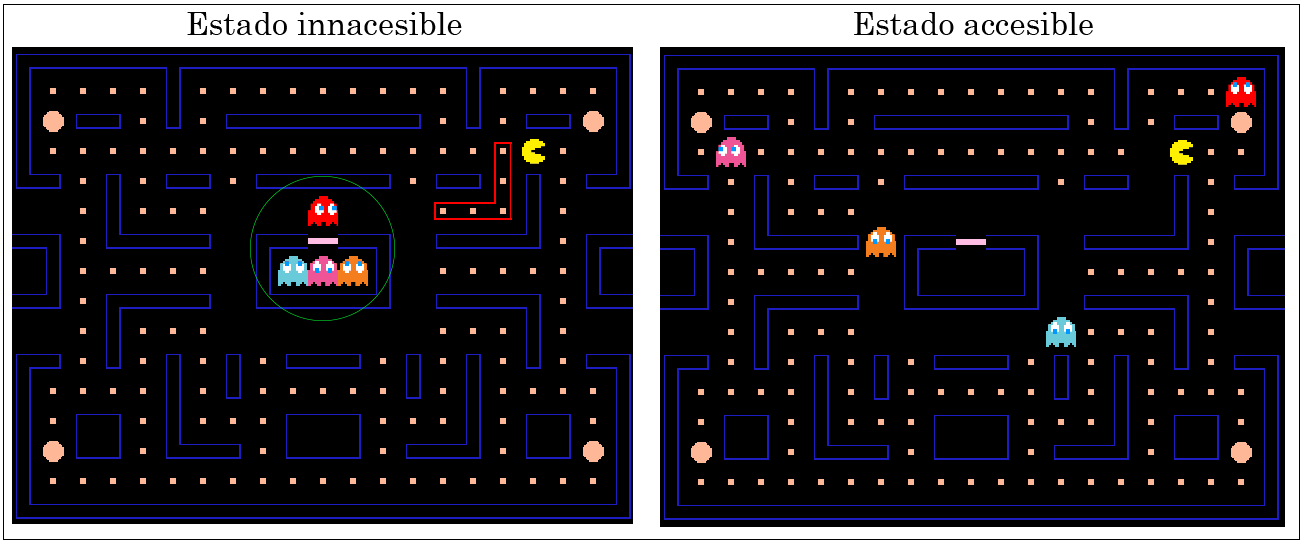
\includegraphics[width=1\textwidth]{images/chapter_3/pacman_states}	
			\caption{Tipos de estados del entorno en el algoritmo DQN}
			\label{fig:pacman_states}
		\end{figure}
		
			
		
		Como se comentó anteriormente, este algoritmo usa redes neuronales para aprender a ejecutar la mejor acción para un estado dado. Se van aplicar las mejoras que se comentan en la sección \ref{cap:3_5} de redes neuronales. En este caso, no se pueden aplicar las mejoras del algoritmo anterior, pues no es una matriz que se pueda dividir el trabajo, si no una red neuronal cuyos pesos varían al ejecutar acciones en estados. 	
		
		
	
		
	
	


\section{Algoritmos Evolutivos}
	\label{cap:3_4}
	Los algoritmos evolutivos son sencillos de paralelizar. Trabajan con poblaciones de individuos que evolucionan a lo largo de las generaciones. Los individuos se someten a operaciones para producir nuevas generaciones. Estas operaciones de cada método son independientes, pues se puede dividir el cálculo entre varios procesos. Los métodos son las siguientes: 
	
	\begin{enumerate}
		\item \textbf{Inicialización.} Dados los parámetros iniciales se crea la población con los individuos deseados. Hay diferentes tipos, con sus respectivas características.
		\begin{itemize}
			\item Binarios. Estos individuos son fáciles de inicializar, pero ralentizan la comunicación entre procesos, debido al gran elevado número de bits que enviar.
			\item Reales. Al igual que los binarios son faciles de inicializar, pero esta vez son más portables, al usar la \textit{base 10} como representación de los números, en vez del sistema binario (0's y 1's). 
			\item Árboles. Más lentos para inicializar y difíciles de tratar. Se usan punteros y aumenta la complejidad al gestionar los punteros.
		\end{itemize}
		
		\item \textbf{Evaluación.} Este es el método que más tiempo de ejecución puede llegar a consumir. Varía dependiendo del tipo de individuo del problema. Como su nombre indica evalúa a todos los individuos dependiendo de una función de fitness, puede ser desde una fórmula matemática hasta una ejecución de un algoritmo en un entorno.
		
		\item \textbf{Selección.} Se seleccionan a los individuos. La aleatoriedad predomina en este método, y dependiendo de la estrategia escogida se puede dar más o menos probabilidad a los más aptos. 
		
		\item \textbf{Cruce.} Todos los individuos se cruzan, y con una cierta probabilidad se eligen a los hijos de estos cruces. Si no se cumple dicha probabilidad no se cruzan los individuos y se dejan como están. Normal mente tendrán un mayor coste temporal que el método anterior.
		
		\item \textbf{Mutación.} Igual que el cruce tiene una probabilidad para mutar. Normalmente es un poco más veloz que el cruce, debido a las estrategias implementadas y que la probabilidad de mutación suele ser menor a la de cruce, provocando una menor tasa de ejecución de la estrategia.
	\end{enumerate}
	
	\begin{flushleft}
		En este trabo se desarrollan los siguientes problemas a optimizar para los tres diferentes individuos implementados.
	\end{flushleft}
	\begin{enumerate}
		\item Los individuos binarios, tienen un intervalo y una precisión como variable de inicialización. Queremos calcular el valor máximo o mínimo para ciertas funciones matemáticas. Los valores \textit{fitness} se calculan con la representación real del cromosoma, que varía dependiendo de la precisión que se le asigna al ejecutar el algoritmo. Por ello hay que convertir la información de binario a real. 
		
		Para estos individuos, el algoritmo se ejecuta bastante rápido, además de alcanzar el máximo global con menos generaciones que los otros dos individuos. La función de evaluación es lineal \textit{O(N)}, debido a la conversión del número binario. Reducir su tiempo de ejecución es desafiante, por el poco coste temporal y el tiempo necesario para enviar/recibir los individuos.		
		\item Los individuos reales, se enfrentan a un problema de mayor complejidad, como es la minimización del retraso total obtenible de una serie de aviones en un aeropuerto. El número vuelos y pistas es variable, y cada vuelo tiene asignado la hora de aterrizaje para cada pista. Hay un tiempo mínimo de separación entre vuelos que aterrizan en cada pista, pues hay que garantizar la seguridad de los pasajeros y la integridad de los aviones. Se puede resolver con vuelta atrás pero tiene un coste exponencial O(\(2^{N}\)). El valor \textit{fitness} tiene coste \textit{O(NumAviones*NumPistas) $\equiv$ O(\(N^{2}\))}. La figura \ref{fig:pev_funcion_ev_2} muestra como se calcula el valor \textit{fitness} de un individuo.
		
		\begin{figure}[!h]
		
		
			\lstset{language=python, 
				breaklines=true, 
				basicstyle=\footnotesize,
				backgroundcolor=\color{lightergray},
				commentstyle=\color{green_comment},}
			\begin{lstlisting}
 fitness=0
 for avion in aviones:
 for pista in range(pistas): # Calculamos TLA para cada pista
 TLA = maximo(TLA(vuelo_anterior) + SEP[vuelo_anterior][vuelo_actual], TEL)
 # Se asigna el vuelo actual a la pista con minimo TLA calculado
 fitness+=(menor_TLA-menor_TEL)^2
 # menor_TEL: menor TEL de ese vuelo con todas las pistas		
			\end{lstlisting}
			\caption{Función de evaluación para los individuos reales en el algoritmo evolutivo}
			\label{fig:pev_funcion_ev_2}
		\end{figure}
		
		El tiempo de ejecución para este problema depende de la función de evaluación, que varía dependiendo del número de aviones y pistas. 
		
		\item Los individuos árbol, han de encontrar una sucesión de acciones en un entorno para maximizar las celdas visitadas en una matriz. Poniendo en contexto, el agente de este problema se encarga de podar un jardín de tamaño \textit{(NxM)} con unos operadores determinados. Estos operadores pueden ser terminales o nodos hoja (nodos del árbol sin hijos) como avanzar podando el cesped o girar a la izquierda (ambos terminales devuelven (0, 0)) y constante, que no altera al agente pero devuelve sus valores (X, Y) para los operadores funciones. Los operadores funciones, expresiones o nodos intermedios (nodos del árbol con al menos un hijo) como Salta(E), operación que provoca que el agente salte y pode la posición destino. O los operadores Progn(E1, E2) y Suma(E1, E2) que aunque no modifiquen al agente aumentan el tamaño del árbol (devuelven la posición de su hijo derecho (E2) y la suma de sus hijos (E1 y E2) respectivamente).
		
		El coste temporal de este algoritmo viene dado principalmente por la función de evaluación. Ejecuta la simulación en la matriz hasta cumplir un determinado número de ticks (acciones realizadas), que es proporcional al número de filas y columnas de la matriz. Aunque las funciones de cruce y mutación también tardan en ejecutarse, debido al control de punteros.
	\end{enumerate}
	
	
	Cada una de las siguientes estrategias MPI se pueden configurar para cada tipo de individuo:

	\begin{enumerate}
		\item Dividir la población en subpoblaciones. Al ejecutar el bucle principal se divide la población entre los procesos para agilizar el trabajo.
		\item Modelo de islas. Se crean varios procesos que ejecutan el algoritmo de manera secuencial.
		\item PipeLine. Se crean varias poblaciones, y cada proceso ejecutado se encarga de ejecutar un método del algoritmo.
	\end{enumerate}
	
	La primera estrategia, representada en la Figura \ref{fig:pev_mpi1}, consiste en dividir la población entre los procesos, se puede paralelizar fácilmente. El \textit{master} recibe de los \textit{workers} las subpoblaciones inicializadas y evaluadas, y comienza el bucle principal del algoritmo, en el cual:
	\begin{itemize}
		\item El \textit{master} se encarga de hacer la selección, y enviarla dividida a los \textit{workers}. Mientras que los \textit{workers} procesan los datos recibidos, el \textit{master} almacena el progreso de los mejores individuos de cada generación.
		\item Los \textit{workers} reciben la selección, la cruzan, mutan y evalúan. Al finalizar estos procesos mandan la subpoblación al \textit{master} para empezar la siguiente iteración.
	\end{itemize}
	
	\begin{figure}[!h]
		\centering
		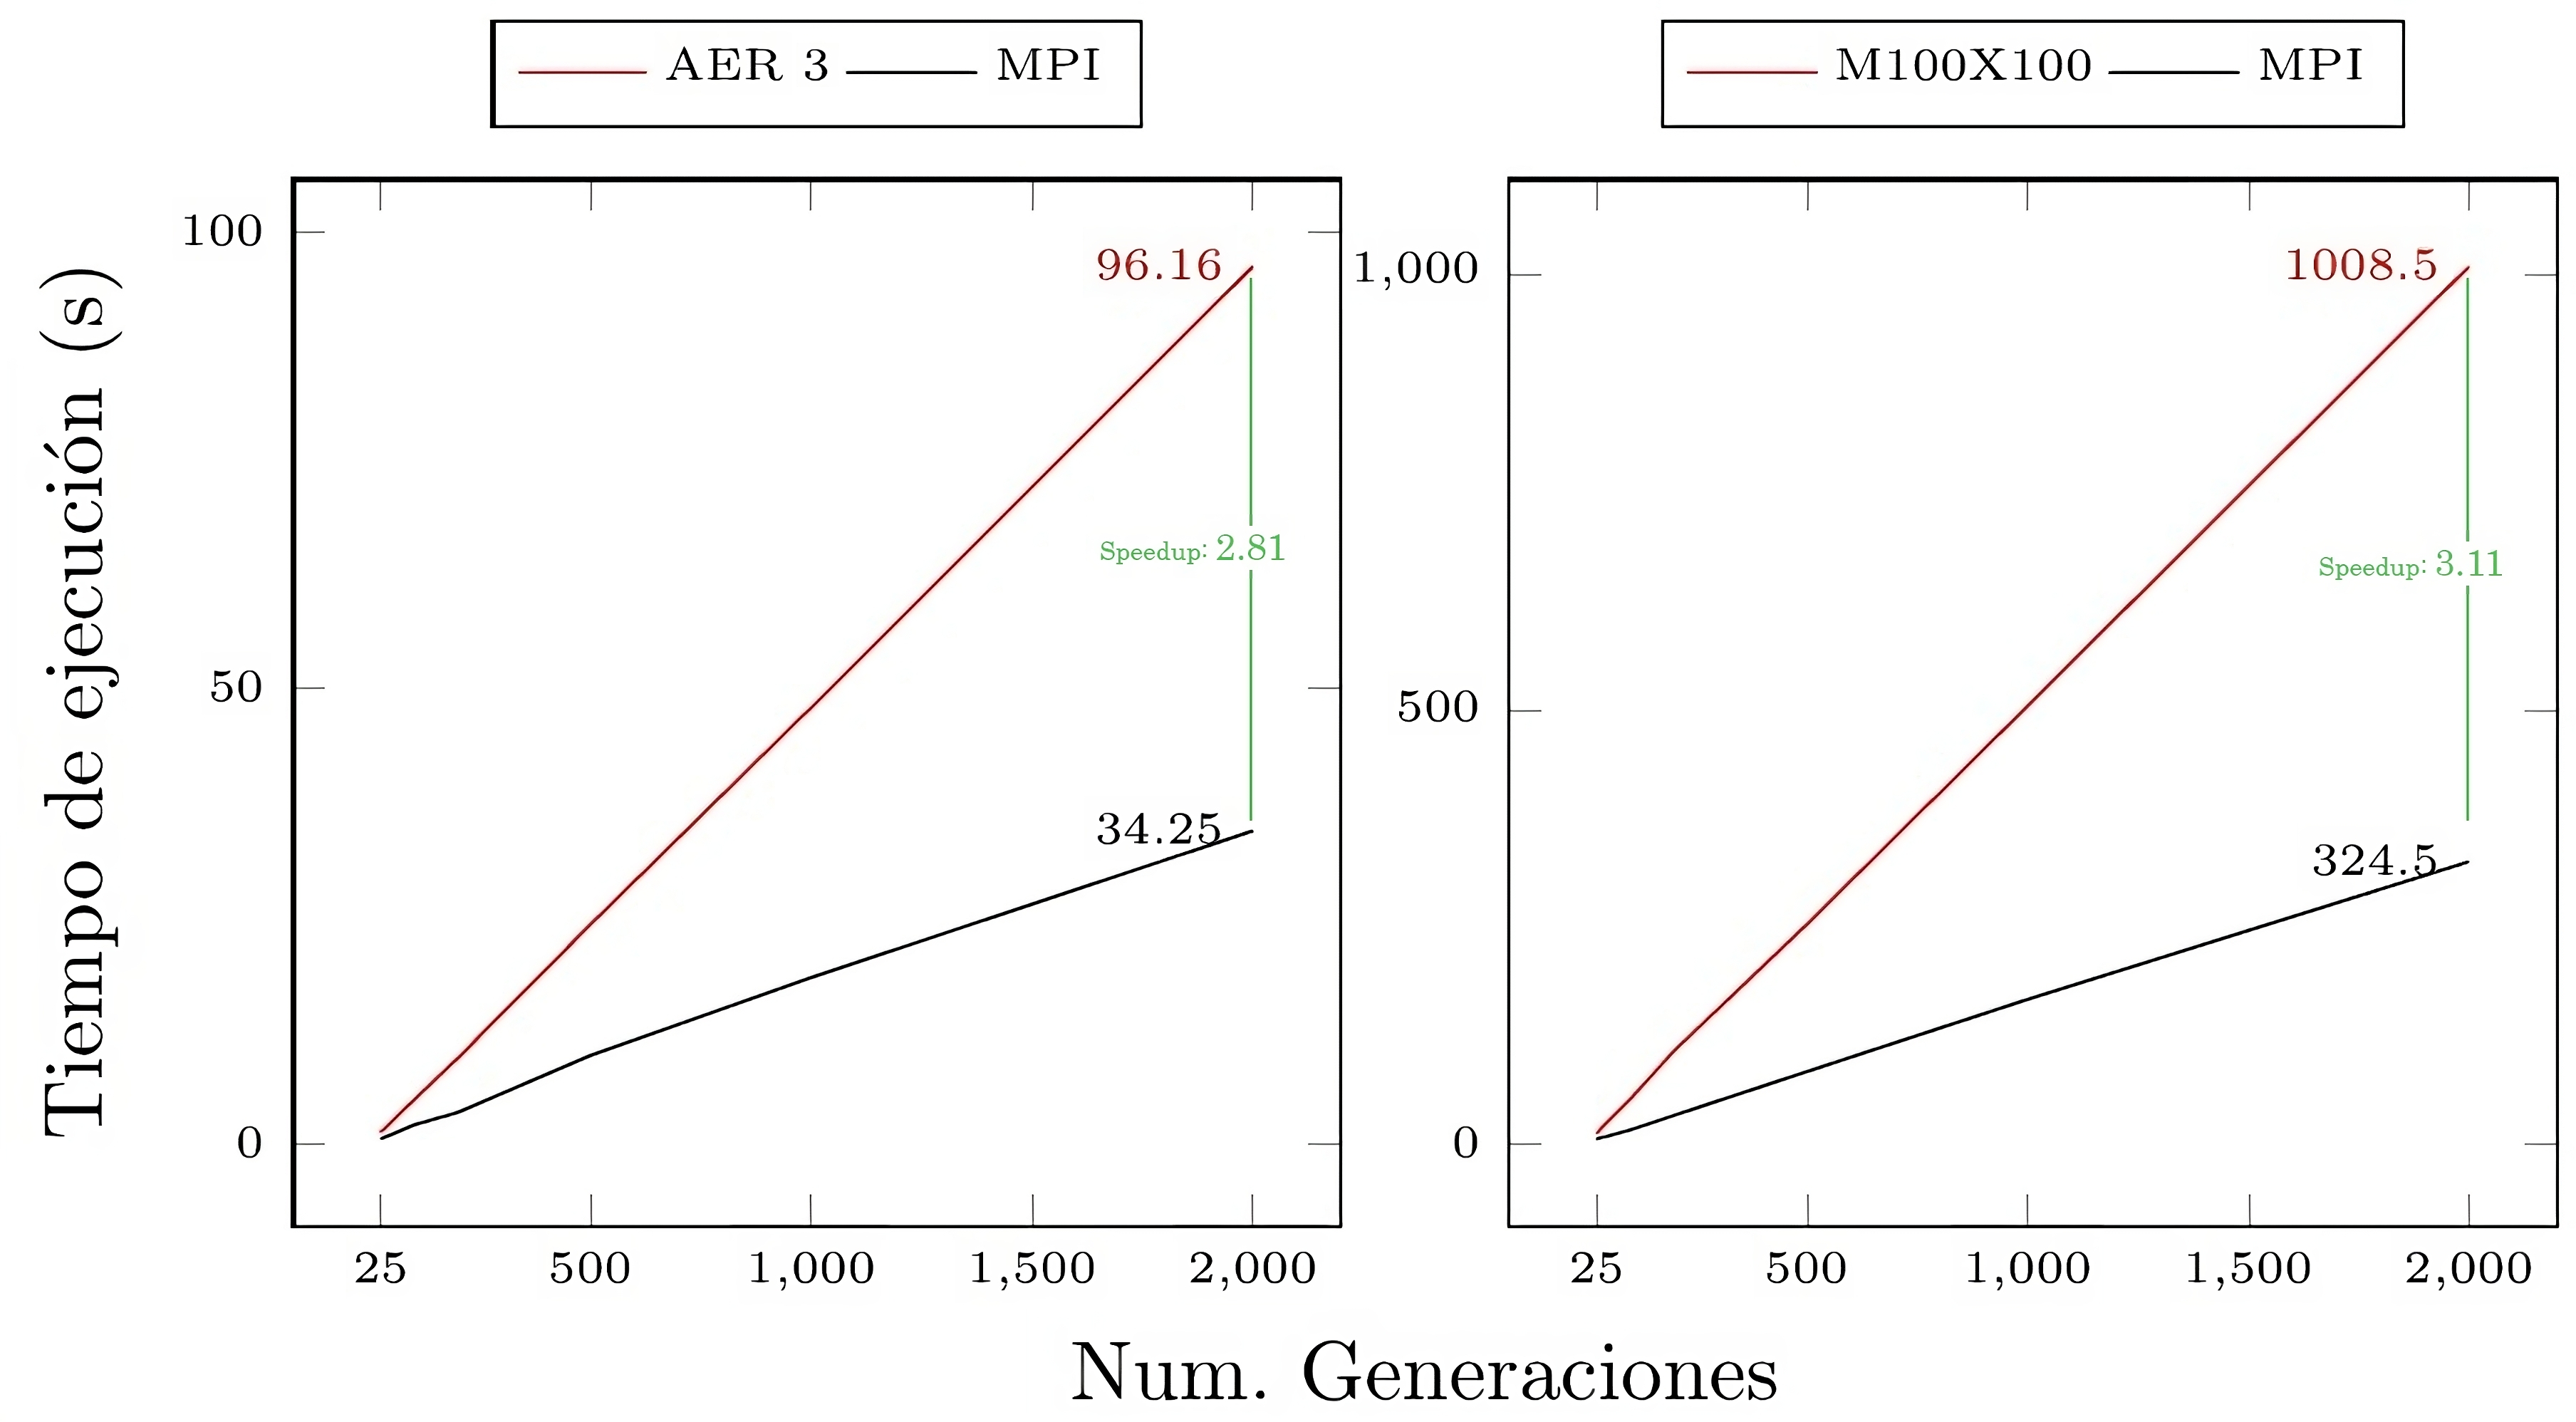
\includegraphics[width=0.65\textwidth]{images/chapter_3/pev_mpi1}
		\caption{Primera estrategia en el algoritmo evolutivo}
		\label{fig:pev_mpi1}
	\end{figure}
	
	Para el modelo de islas (segunda estrategia), se aplica la estrategia que se ha desarrollado anteriormente para otros algoritmos. Cada proceso ejecuta el algoritmo básico, dividiendo la población general en los procesos ejecutados. Con este modelo se reduce la comunicación entre los procesos, pues al contrario que la estrategia anterior, no se reserva funcionalidades para diferentes procesos, si no que cada proceso se encarga de ejecutar todas las funciones para que su subpolación evolucione correctamente. Cada cierto tiempo se reinicia la población con los mejores individuos generales (de todos los procesos). Los tipos de comunicación se representaN en la Figura \ref{fig:pev3_mpi2}, y son los siguientes: 

	\begin{itemize}
		\item Estrella. El \textit{master} se posiciona en el centro y solo hay comunicaciones \textit{Master-Worker} para almacenar los mejores individuos de cada subpoblación.
		\item En red. No hay proceso \textit{master}, todos los procesos ejecutan el algoritmo. Al finalizar una iteración todos los procesos se comunican entre sí, mandando los mejores individuos para el reinicio de la población.
		\item En anillo. Igual que el anterior, pero esta vez no se comunican todos los procesos. La comunicación, como nu nombre indica se hace con topología circular, cada proceso se comunica con su predecesor y sucesor.
	\end{itemize}
	
	\begin{figure}[!h]
		\centering
		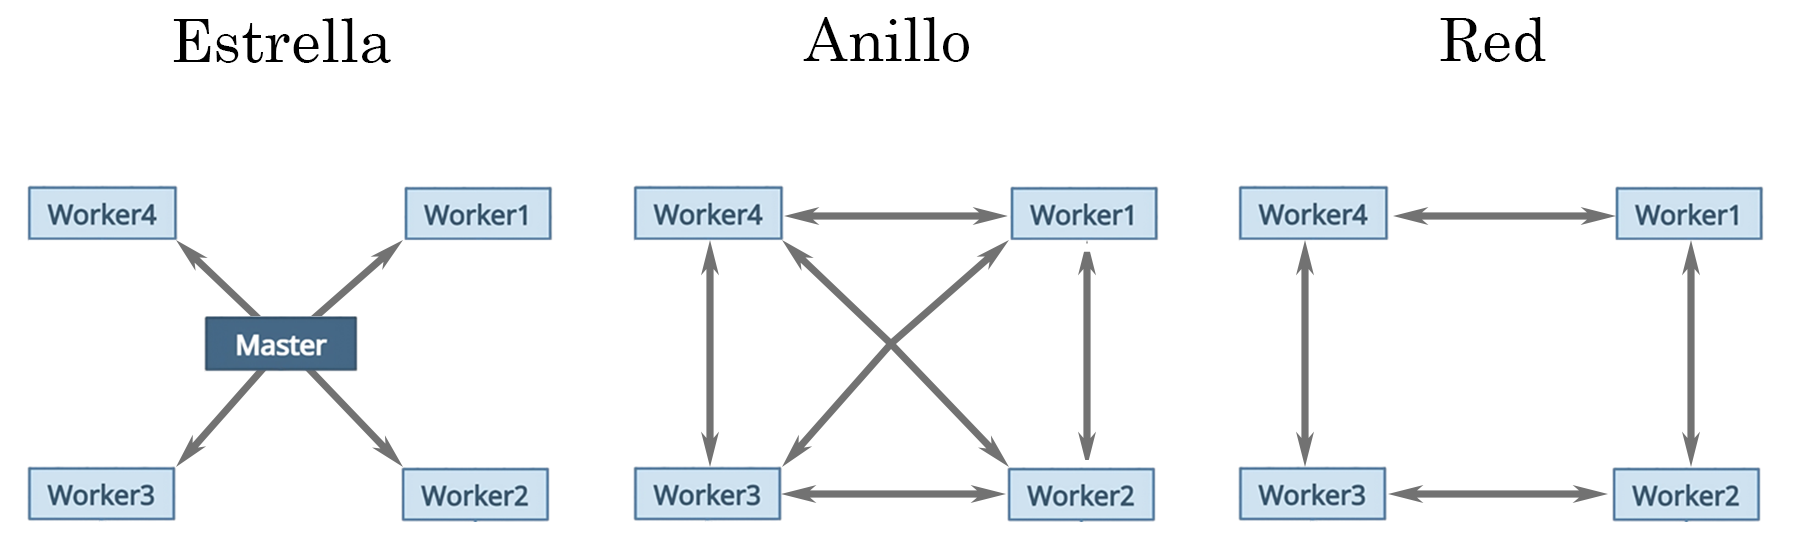
\includegraphics[width=\textwidth]{images/chapter_3/pev_mpi2}
		\caption{Segunda estrategia en el algoritmo evolutivo}
		\label{fig:pev3_mpi2}
	\end{figure}
	
	Segmentar el algoritmo entre los procesos (tercera estrategia, representada en la Figura \ref{fig:pev_mpi3}), provoca un flujo constante de generaciones. Como hay cinco métodos principales se necesitan, al menos, cinco procesos, incluyendo al \textit{master}, que se encarga de inicializar y evaluar las cuatro distintas poblaciones que se van a ejecutar al mismo tiempo. Al principio, todos los procesos \textit{workers} están en espera de recibir una población para ejecutar sus operaciones. El primer \textit{worker} se encarga de la selección y se despierta en la segunda iteración al recibir la primera población inicializada por parte del \textit{master}. Una vez ha ejecutado las cuatro selecciones de las poblaciones que el \textit{master} le envía, empieza a recibir las poblaciones del último \textit{worker}. Los otros tres \textit{workers} se encargan del cruce, mutación y el último de la evaluación, despertándose en la tercera, cuarta y quinta iteración respectivamente por parte de su \textit{worker} predecesor. El último \textit{worker} finaliza una generación al enviar la evaluación de la población mutada al \textit{worker 1}, encargado de realizar la selección. No hay conflicto con el \textit{master}, ya que, como se mencionó anteriormente en este párrafo, este crea cuatro poblaciones (terminando en la iteración cuatro, mientras que la primera evaluación del último \textit{worker} se finaliza en la iteración cinco), y al finalizar su trabajo pasa a un estado de recepción de los mejores individuos. Si se ejecutan \textit{100} generaciones, esta estrategia evoluciona cuatro poblaciones distintas, en \textit{104} generaciones en total, de las cuales \textit{96} se ejecutan las cuatro poblaciones simultaneamente.
	
	
		
	\begin{figure}[!h]
		\centering
		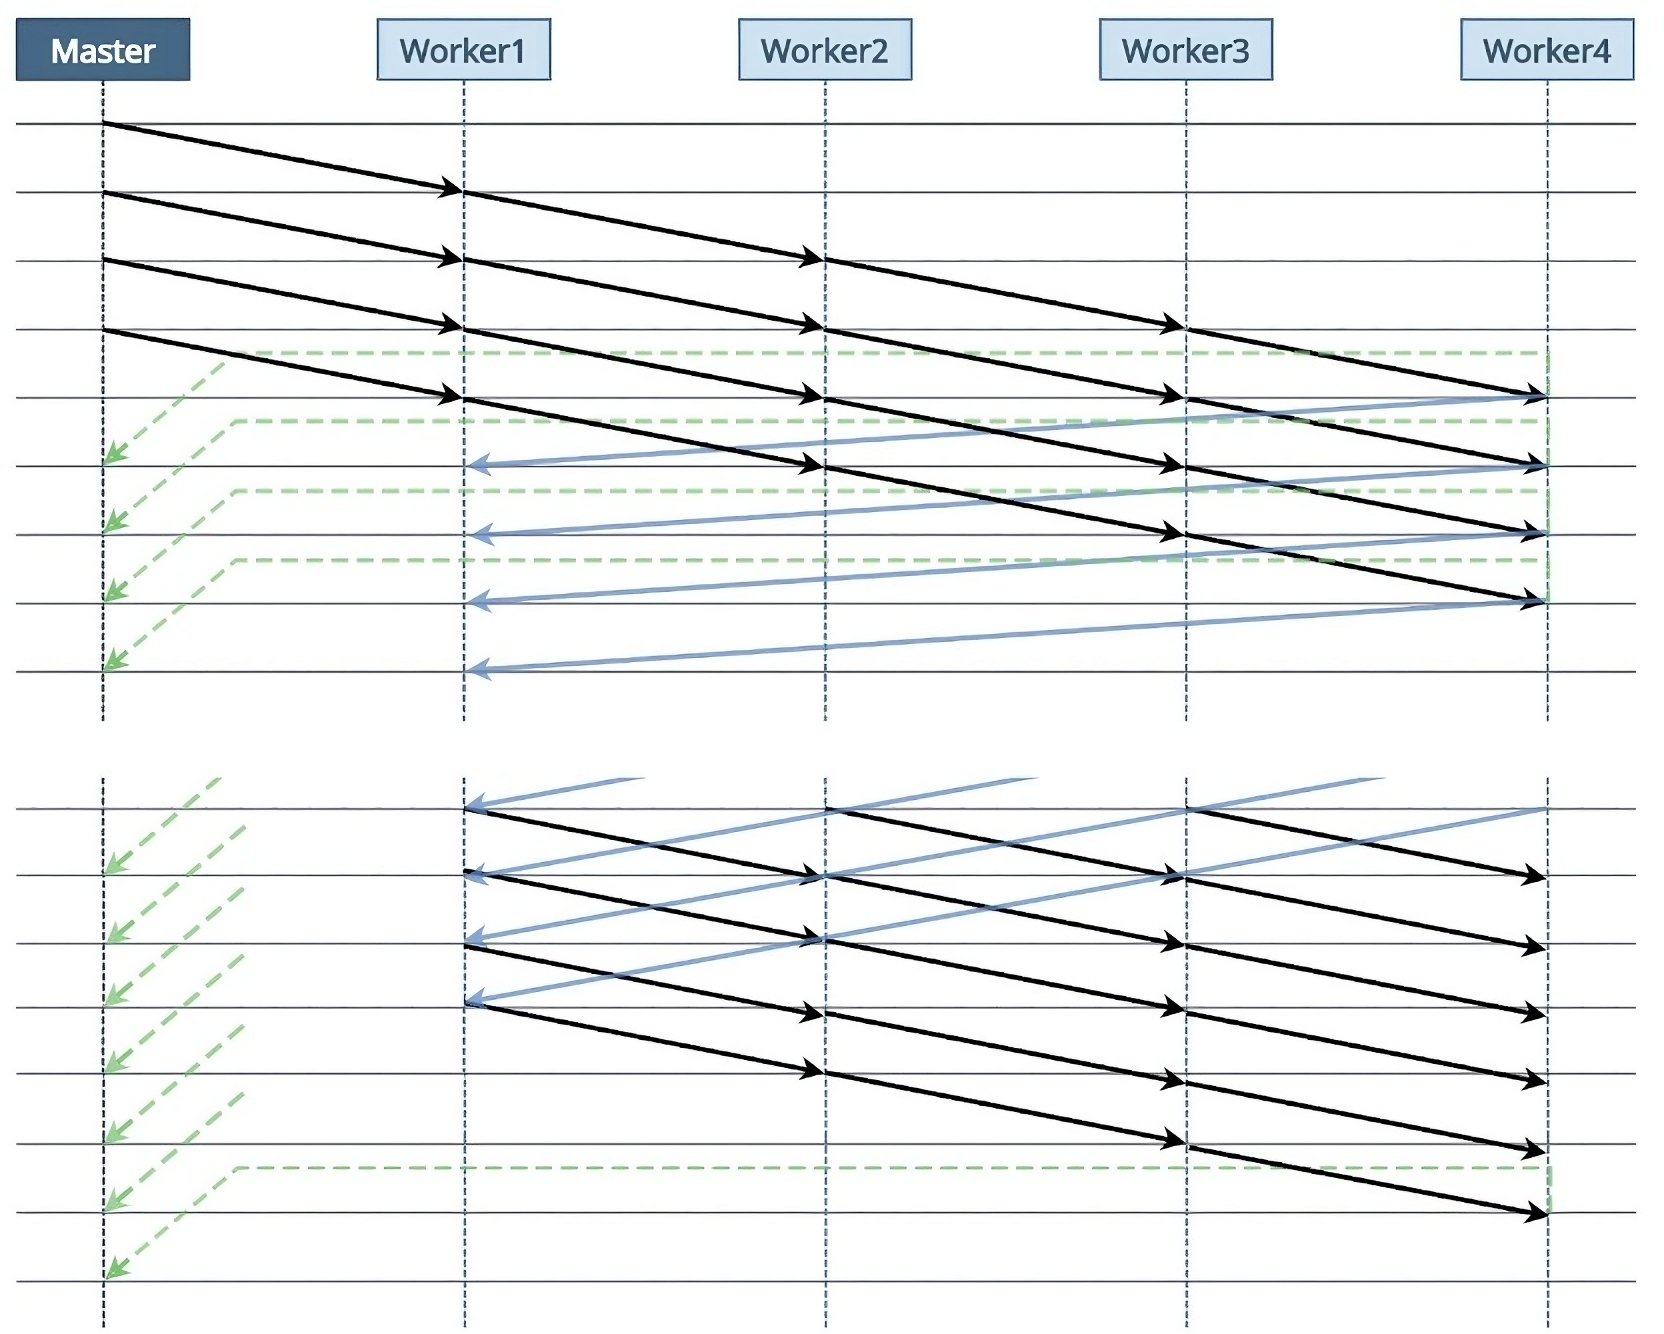
\includegraphics[width=0.65\textwidth]{images/chapter_3/pev_mpi3}
		\caption{Tercera estrategia (PipeLine) en el algoritmo evolutivo }
		\label{fig:pev_mpi3}
	\end{figure}

	El tiempo de ejecución de esta estrategia es proporcional al número de generaciones ejecutadas multiplicado por el proceso que más tiempo tarda en ejecutarse. Por lo que se puede reducir el tiempo de ejecución si comprobamos que métodos tardan más, añadiendo más procesos para reducir la carga de trabajo. Por ejemplo en los individuos reales y árboles el método que más tiempo consume es la evaluación de individuos, por lo que conviene añadir más procesos para reducir así el tiempo de ejecución.
	
	
	
	

\section{Redes Neuronales}
\label{cap:3_5}
%\label{sec:redes_neu}	
	Esta poderosa herramienta de aprendizaje supervisado, está diseñada para reconocer patrones complejos y realizar diversas tareas. Aprende con un proceso iterativo de entrenamiento, ajustando las conexiones entre neuronas. Este proceso secuencial es complejo de paralelizar. Al finalizar una predicción, el modelo se tiene que actualizar propagando hacia atrás.
	
	Nos centramos en la técnica de predicción. Para comenzar, vamos a crear una red neuronal que aprenda a predecir el Índice de Masa Corporal (IMC) de una persona. Cada individuo está formado de dos variables, la altura en centimetros y el peso el kilogramos. Para moldear la red neuronal a los individuos, la capa de entrada se estructura con dos neuronas, una para cada variable, y la salida es el IMC, por lo que la capa de salida es una única neurona. La capa de entrada y salida no varían, pero la capa oculta se puede modificar libremente, aumentando el tiempo en la fase de entrenamiento.
	
	
	Como en algunos de los algoritmos anteriores, necesitamos encontrar la mejor configuración de los hiper-parámetros. En las redes neuronales solo hay uno. La tasa de aprendizaje, controla la magnitud de los ajustes a realizar en los pesos de las neuronas durante el proceso de entrenamiento. Específicamente, determina cuánto deben cambiar los pesos en respuesta al error cometido a predecir un individuo.
	
	
	Por ello, diseñamos una estrategia para encontrar la mejor tasa de aprendizaje para una red neuronal en concreto. El proceso \textit{master} envía intervalos de tasas de aprendizaje a todos los procesos \textit{workers} ejecutados, para que estos ejecuten el algoritmo y envíen el sumatorio de errores obtenidos en la predicción. La inicialización de los pesos, normalmente es aleatoria, pero para hacer más igualitario el calculo de los errores, todos los procesos inicializan la red neuronal con los mismos pesos.
	
	
	\noindent Las estrategias MPI realizadas son las siguientes:
	\begin{enumerate}				
		\item PipeLine. Como en el algoritmo anterior, pero esta vez con un flujo de mensajes bidireccional.
		\item Dividir el trabajo entre los procesos.
	\end{enumerate}
	
	Segmentar el proceso de entrenamiento puede llegar a ser beneficioso. Cada proceso se encarga de una capa de la red neuronal, siendo el \textit{master} el encargado de enviar individuos de la población categorizada. El último \textit{worker} controla la capa de salida, con las etiquetas de los individuos, calcula el error y lo propaga hacia atrás. Para el correcto funcionamiento, hay que crear un buen diseño para tener un flujo constante de mensajes, los cuales pueden ser síncronos, es decir, que esperan a recibir los mensajes, o asíncronos, siendo estos últimos solamente admisibles en la etapa de recibir mensaje de una propagación hacia atrás anterior y enviar mensaje hacia adelante del individuo actual. La figura \ref{fig:redneumpipipe} muestra dicho flujo y el trabajo de los procesos es el siguiente:	
	
	
	\begin{enumerate}
		\item El \textit{master} envía un número proporcional de individuos a los procesos en ejecución. Luego, antes de enviar otro individuo, entra en un bucle en el cual recibe el error de un individuo ya enviado, actualizando sus neuronas, y envía otro individuo. Para finalizar recibe el mismo número de errores (actualizando las neuronas) que individuos envió al principio.
		\item El último \textit{worker} solo recibe las predicciones y calcula el error.
		\item Los \textit{workers} de la capa oculta tienen un proceso más complejo. Primero, reciben un número de individuos proporcional a su \textit{id}, los procesan y envían. Después entran en un bucle en el cual:			
		\begin{itemize}
			\item Reciben de la capa siguiente: los errores, actualizan sus pesos y lo propagan enviando lo a la capa anterior.			
			\item Reciben de la capa anterior: los nuevos individuos, procesan y propagan hacia adelante.
		\end{itemize}		
		
	\end{enumerate}
	
	\begin{figure}[!h]
		\centering
		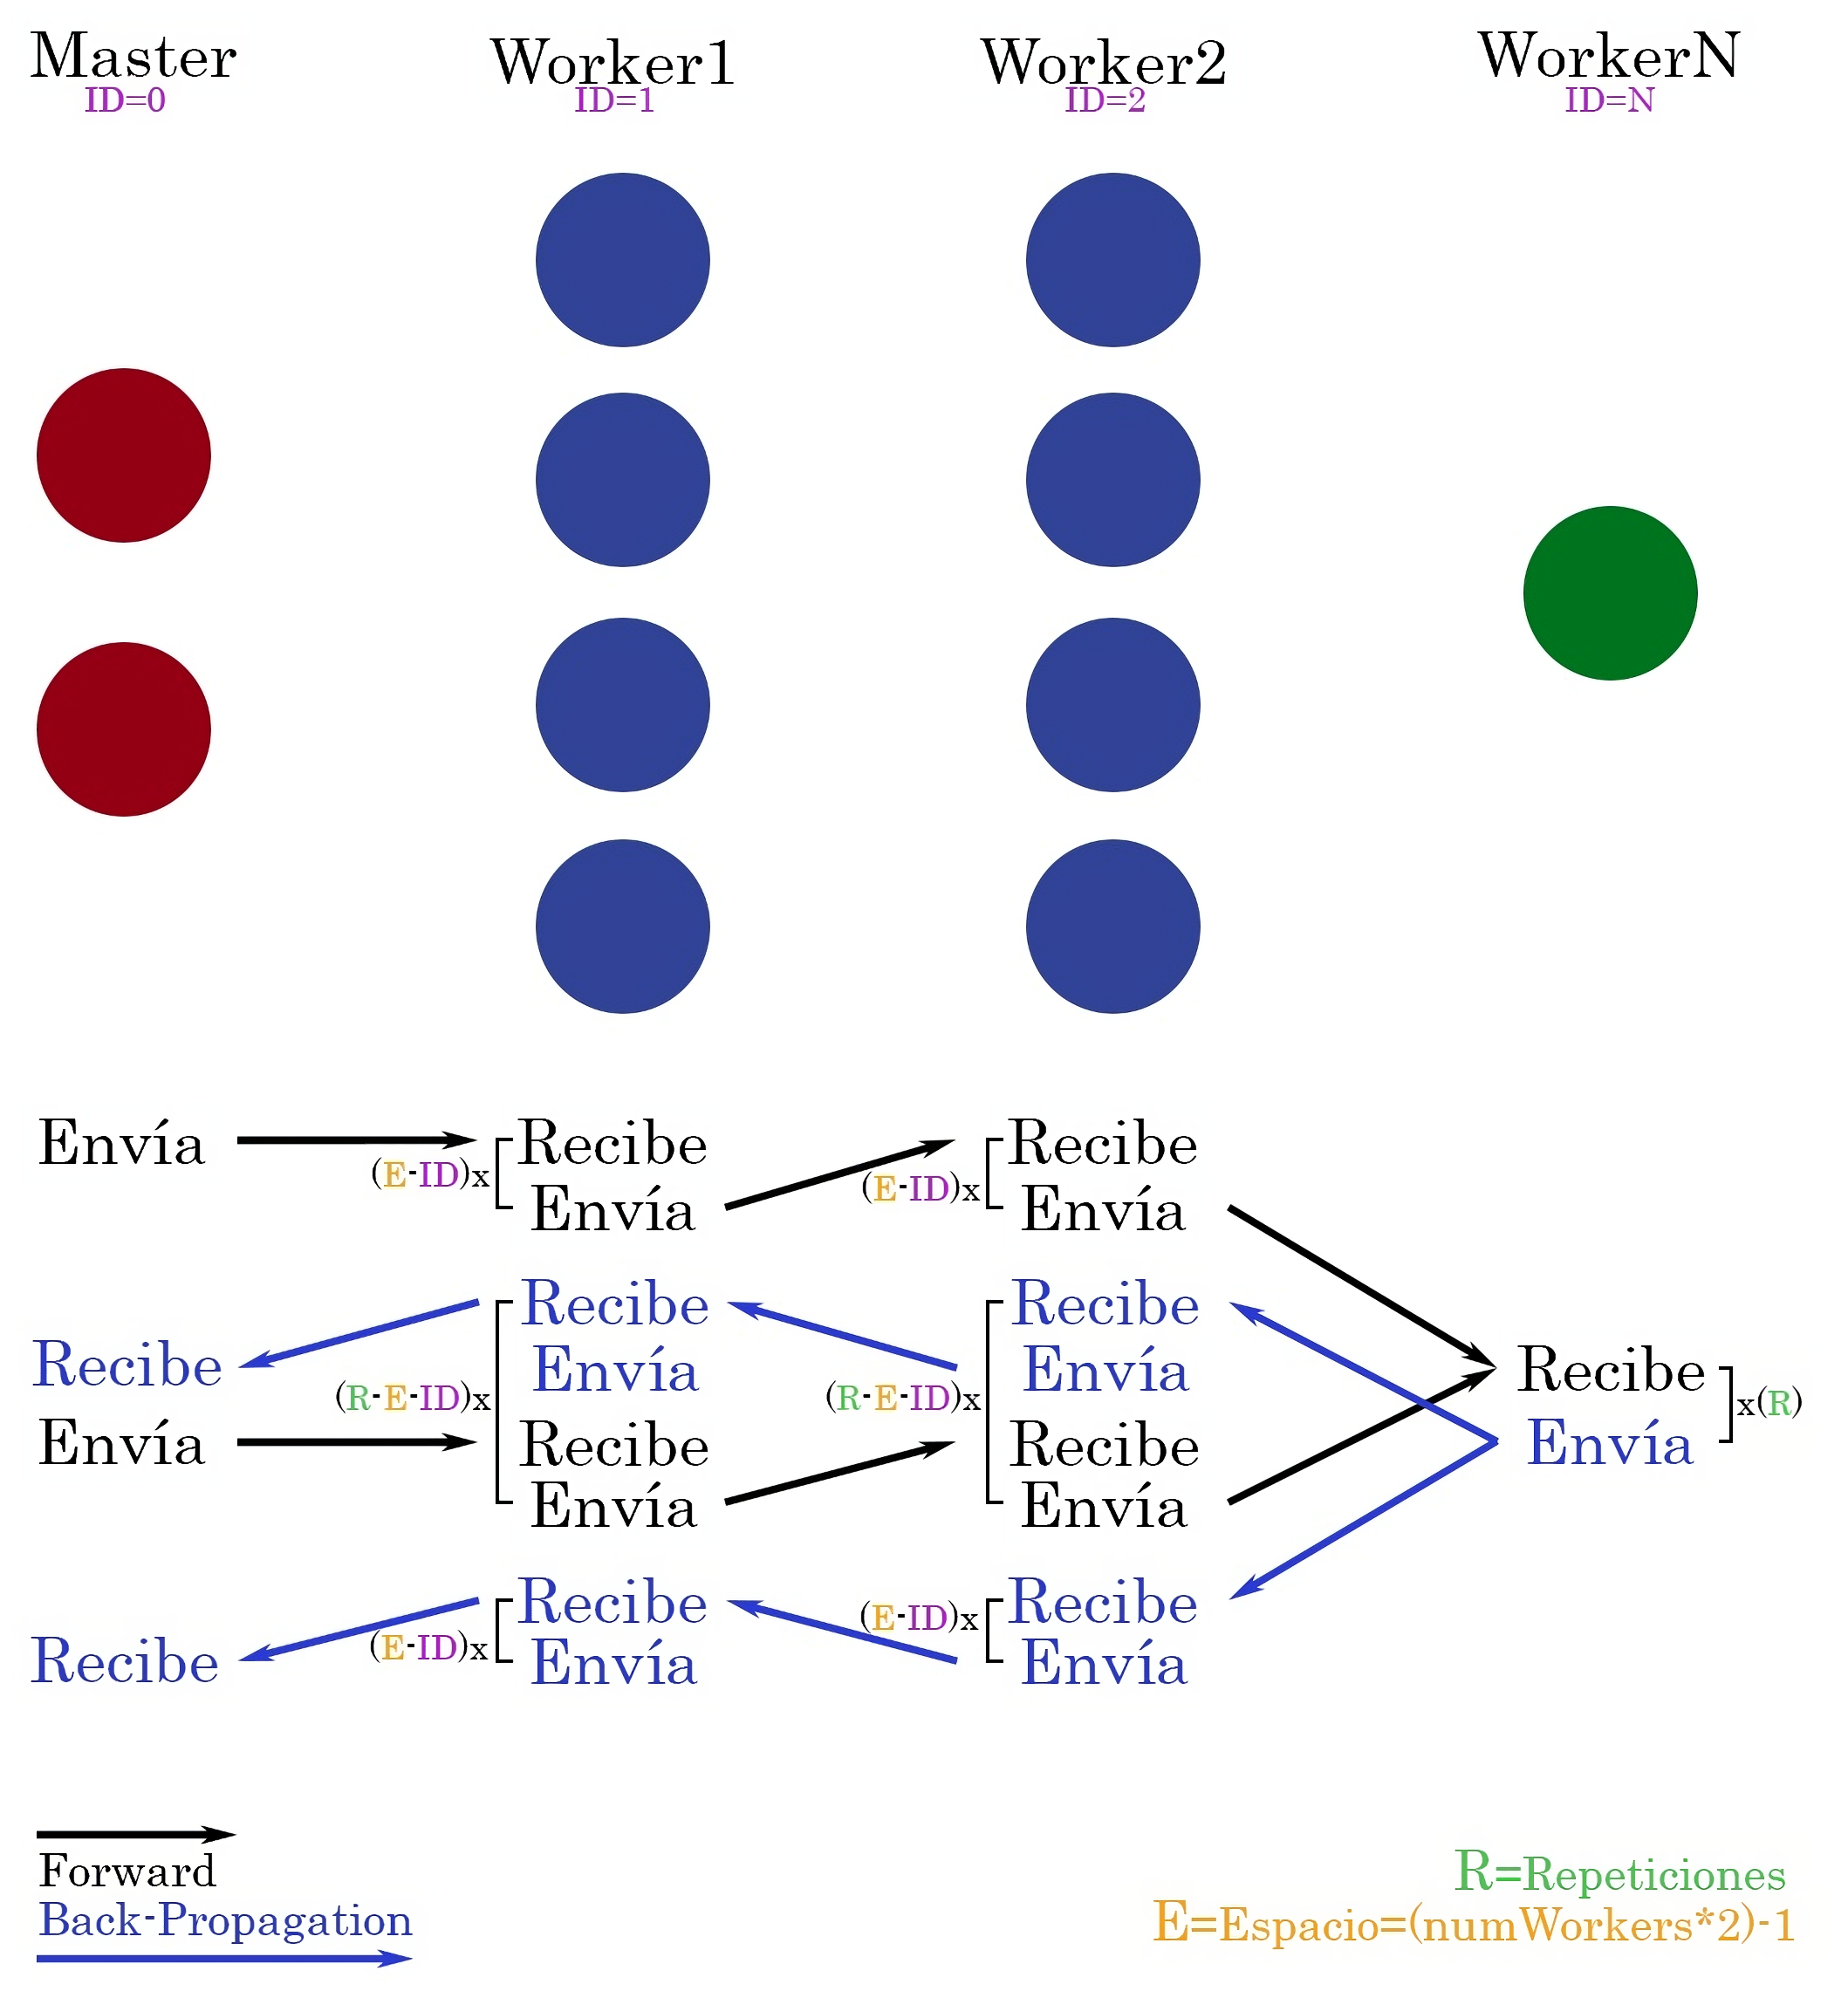
\includegraphics[width=0.55\textwidth]{images/chapter_3/redneu_mpi2}
		\caption{Primera estrategia en el algoritmo Red Neuronal}
		\label{fig:redneumpipipe}
	\end{figure}
	
	Al ser un proceso iterativo, en el cual el modelo va aprendiendo en la fase de entrenamiento, a primera vista, dividir la población entre procesos (segunda estrategia) no parece ser beneficioso para el correcto aprendizaje de la red. Sin embargo, en redes neuronales hay un proceso llamado \textit{fine tuning} \cite{malladi2023fine} que consiste en entrenar una red neuronal, con unos pesos ya calculados. Basándonos ligeramente en esta técnica, podemos implementar una mejora en la cual dividamos la población inicial entre procesos y, en paralelo, ejecutamos la fase de entrenamiento. Una vez finalizadas, el \textit{master} recibe los pesos de cada \textit{worker} y hace la media. Cuanto más grande sea la red neuronal mayor será -a priori- el rendimiento.
		
	Las neuronas varían sus pesos para adaptarse a las variables recibidas. Para predecir un individuo, todas las neuronas trabajan en conjunto. Lo que supone que una neurona perteneciente a una red de menor tamaño tendrá más relevancia en comparación con una neurona en una red de mayor escala. Esto plantea un interrogante: ¿es posible paralelizar el trabajo de una red neuronal de gran escala y conservar o reducir el porcentaje de error al predecir individuos? Para ponerlo a prueba hay que probar varias estrategias de agrupaciones en la población que se va a utilizar para entrenar la red neuronal, además de tener en cuenta la inicialización de los pesos.
	
	\begin{enumerate}
		\item Misma población en todos los procesos. 
		
		\begin{itemize}
			\item Si cada proceso tiene la misma población y los mismos pesos en la red, si reduce el tiempo de ejecución, pero no mejora la predicción. Sería como ejecutar el algoritmo sin paralelizar, pero con menos iteraciones, pues se ejecutan en los procesos la misma ejecución y la media no varía con respecto a los resultados obtenidos.
			\item Inicializando las distintas redes neuronales con pesos diferentes, puede predecir correctamente para este problema en particular pero no tener unos buenos resultados de manera global o viceversa. Además, depende de la aleatoriedad, pues el porcentaje de errores en una ejecución puede variar bastante con respecto a otra. 
		\end{itemize} 
		
		\item Diferentes poblaciones para cada proceso. 
		
		Esta estrategia suena mejor que la anterior. Al no haber intersección de poblaciones en los procesos ejecutados, los valores de los pesos se modificaran de diferente forma y puede que al hacer la media la red se estructure de forma que se obtenga un correcto funcionamiento. La inicialización de los pesos no provoca una gran diferencia, al contrario que mantener la misma población para todos los procesos. Pero conviene probar ambas inicializaciones.	
		
		
	\end{enumerate}	
	
	

	